\documentclass[../main]{subfiles}
\ifSubfilesClassLoaded{
    \dominitoc
    \tableofcontentsfile
	\pagenumbering{arabic}
    \setcounter{page}{1}
	\addbibresource{../Biblio/biblio.bib}
}{}
\begin{document}
\chapter{Analyse de l'auto-organisation de CxSOM sur des cartes en une dimension}\label{chap:analyse}
\graphicspath{{06-Analyse/figures},{./figures}}
\minitoc


Nous avons proposé un modèle de connexions de cartes auto-organisatrices au sein d'une architecture complète s'appuyant sur une recherche de consensus entre BMUs. Nous avons vu dans le chapitre précédent que ce consensus permet de définir un BMU.
Dans ce chapitre, nous nous intéressons aux mécanismes d'auto-organisation des poids occurrant dans des cartes. 
Nous étudions encore ici les cartes en une dimension~; nous ouvrirons l'étude aux cartes en deux dimensions au chapitre suivant.





\section{Méthode expérimentale}

Nous utiliserons en premier lieu des modèles géométriques d'entrées. 
Ces modèles nous permettent de maîtriser les dépendances sur des modalités en basse dimension et ainsi de visualiser les liens entre organisation et apprentissage. 
Cela nous permettra également de mesurer l'apprentissage de cette dépendance connue au sein des structures de cartes.

\subsection{Modèle d'entrées géométriques}

Rappelons la définition des entrées multimodales~: il s'agit d'un ensemble d'entrées $\mathbf{\inpx} = (\inpx\m{1}, \cdots, \inpx\m{n})$
Nous représentons la dépendance entre entrées en choisissant une variable latente du modèle $U$ telle que :
$$ \forall i, \inpx\m{i} = f\m{i}(U) + \epsilon\m{i}$$
avec $\epsilon\m{i}$ un bruit sur les entrées.
La dépendance entre modalités est définie par la dimension choisie pour $U$.
Une variable $U$ en une dimension paramètre des points placés sur une courbe en une dimension~; $U$ en 2 dimensions paramètre une surface 2D. 

Dans cette série d'expériences, nous étudions un modèle dans lequel chaque modalité est unidimensionnelle. Chaque modalité correspond à une coordonnée d'un objet géométrique en $K$ dimensions, avec  $K$ le nombre de cartes. Afin de définir une dépendance entre entrées, nous les prenons sur une variété de dimension inférieure, $k$,  paramétrée par $U \in [0,1]^k$.
Ce modèle est général~: au pire, $U$ correspond à la dimension totale des entrées. 
Par ailleurs, de nombreux modèles d'entrées réelles se placent sur une variété (\emph{manifold}) de dimension réduite, comme nous l'avions vu au chapitre \ref{chap:repr} pour des images d'un même objet 3D vu par différents angles. Le choix d'un modèle d'entrées géométriques situées sur une variété de dimension inférieure est donc justifié comme modèle expérimental simplifié.
Dans ce chapitre, nous considérons des architectures de deux et trois cartes et prenons donc des entrées de dimension totale $K = 2$ et $K = 3$.


Dans une architecture de deux cartes, nous considérons d'abord des points pour lesquels $U$ est en une dimension~: ils sont situés sur une courbe du plan 2D.
Nous reviendrons d'abord  sur les conclusions de l'expérience présentée au chapitre représentation, sur des données disposée en cercle (\textbf{A}). L'intérêt de cette courbe est que la disposition est symétrique~: toute entrée $X^{(1)}$ correspond à deux valeurs possibles pour $X^{(2)}$ et inversement.
Nous testerons ensuite si les observations réalisées sur cette disposition d'entrées se retrouve dans d'autres dispositions listées ci-dessous, représentées en figure~\ref{fig:input_list}~:
\begin{itemize}
	\item Une entrée est fonction de l'autre~: $\inpx\m{2} = cos(\inpx\m{1})$~(\textbf{B})
	\item Entrées identiques (cas dégénéré). Ces points sont toujours sur une courbe 1D, mais leur dépendance est bijective.~(\textbf{C})
	\item Entrées sur une courbe de Lissajous (\textbf{D})~: une entrée $\inpx\m{1}$ correspond à 4 à 6 valeurs de $\inpx\m{2}$ et inversement.
	\item Entrées totalement indépendantes, prises aléatoirement dans un carré $[0,1]^n$~(\textbf({E})). $U$ est alors une variable 2D correspondant aux entrées.
	\item Une carte de Kohonen classique a comme propriété d'être résistante au bruit des données. Ainsi, une carte 1D se dépliant sur un anneau fin en 2D apprendra d'abord la représentation du cercle. Nous voulons vérifier comment cette propriété se vérifie sur l'apprentissage de données par plusieurs cartes~; nous prendrons ainsi des points sur un anneau \textbf{(F)}. $U$ est ici en une dimension, et chaque dimension est bruitée.
\end{itemize}


Sur ces différents jeux d'entrées, nous étudierons l'organisation après apprentissage de deux cartes connectées réciproquement et tracerons les représentations. Nous suivons la méthode expérimentale et les représentations élaborées au chapitre \ref{chap:repr}.
Dans un premier temps, nous étudions des architectures de deux cartes 1D, ce qui nous permettra de mieux comprendre certains mécanismes d'organisation.
Nous étendrons ensuite notre étude à des architectures de 3 cartes en une dimension, toutes connectées.

Nous étendrons ensuite notre étude à des modèles d'architectures de trois cartes. Nous prendrons deux configurations d'entrées : 
\begin{itemize}
	\item Les entrées sont dans un plan 2D pivoté en trois dimensions
	\item Les entrées sont sur un cercle en 2D, pivoté en trois dimensions
\end{itemize}

Dans ces deux cas, la connaissance de deux des entrées et du modèle détermine la valeur de la troisième entrée. Nous étudierons ces configurations dans un cadre de prédiction d'entrées~: nous donnons en entrées $X\m{1}, X\m{2}$ à la structure et regardons si la valeur de $X\m{3}$ correspondante est correctement prédite par l'architecture. Une bonne prédiction témoignera de l'apprentissage du modèle d'entrées par l'architecture de cartes.
Les architectures de cartes en deux dimensions seront traitées par la suite au chapitre~\ref{chap:analyse2D}.

\begin{figure}
	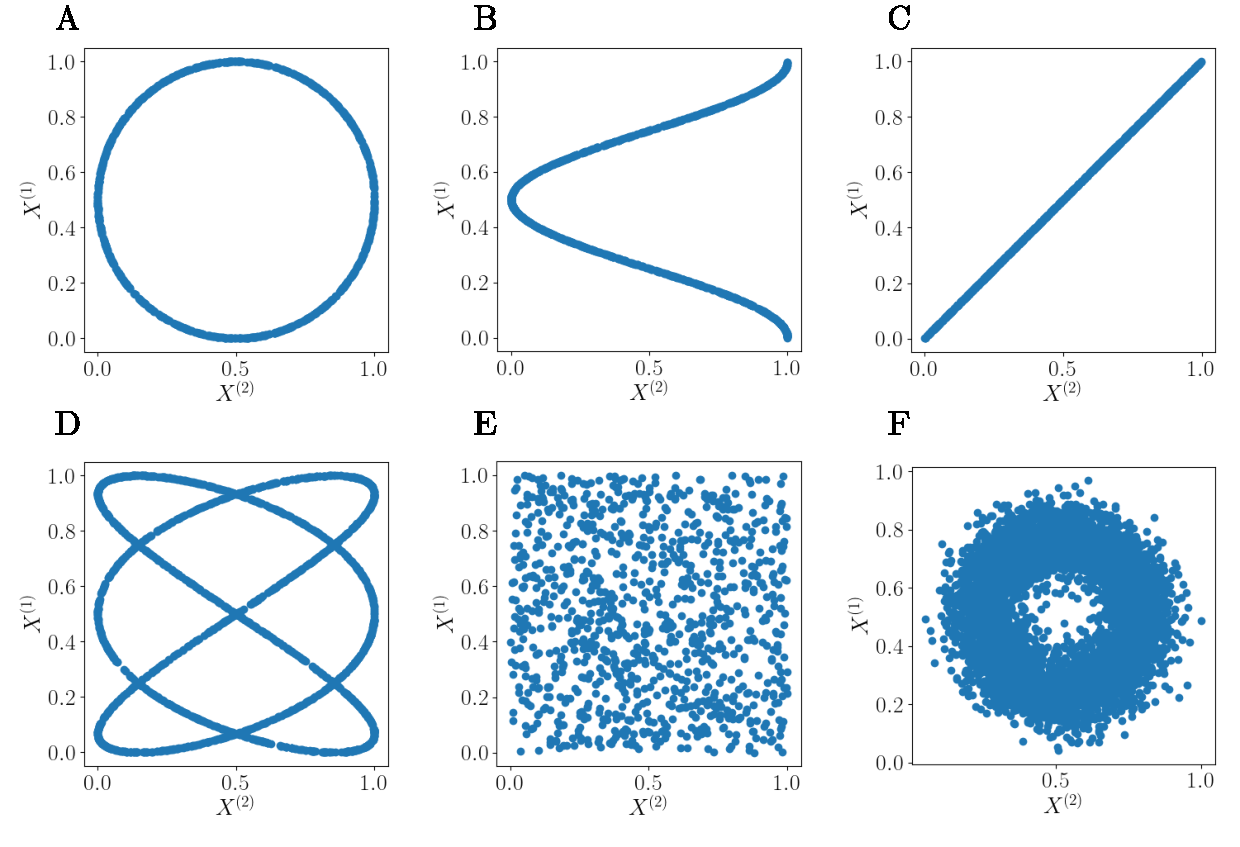
\includegraphics[width=\textwidth]{inputs/inputs.pdf}
	\caption{Dispositions d'entrées en deux dimensions. $M\m{1}$ prend en entrée l'ordonnée $\inpx\m{1}$ et $M\m{2}$ prend en entrée l'abscisse $M\m{2}$. \label{fig:input_list}}
\end{figure}

\begin{figure}
	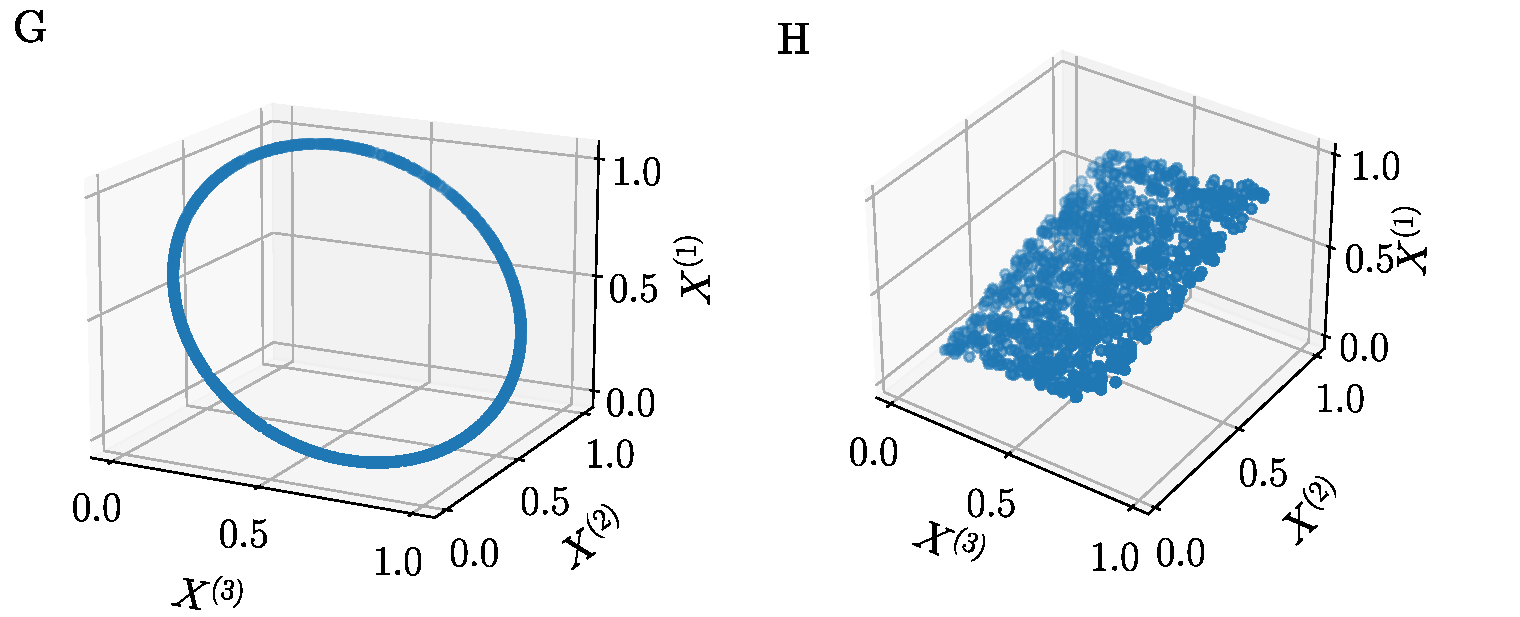
\includegraphics[width=\textwidth]{inputs/inputs_3D.pdf}
	\caption{Dispositions d'entrées en deux dimensions. $M\m{1}$ prend en entrée l'ordonnée $\inpx\m{1}$ et $M\m{2}$ prend en entrée l'abscisse $M\m{2}$. \label{fig:input_list}}
\end{figure}


\subsection{Matériel}

Les expériences présentées ici ont été développées en C++ en s'appuyant sur la librairie CxSOM \footnote{\url{https://github.com/HerveFrezza-Buet/cxsom}}, développée au sein de notre équipe.
Cette librairie permet d'implémenter des cartes de Kohonen simples ainsi que des architectures CxSOM par le modèle que nous avons présenté.
Cette librairie s'interface avec python par un module pycxsom afin de faciliter les représentations et manipulation des cartes pendant et après l'apprentissage. Elle cherche à paralléliser au maximum les opérations indépendantes. Par exemple, la phase d'apprentissage des cartes reste séquentielle car le calcul des valeurs des poids pour l'itération $i$ dépend de $i-1$, mais toutes les opérations de tests dans lesquelles le temps n'intervient pas tournent en parallèle.
Notons que la gestion du consensus lors de la relaxation passe également par des mécanismes locaux aux cartes dans notre implémentation. Nous devons en effet vérifier lors de chaque pas de relaxation si les cartes ont atteint un consensus. Pour cela, chaque carte envoie un signal supplémentaire aux cartes voisines indiquant si son BMU a été modifié. Lorsque qu'une carte reçoit de toutes ses voisines que leur BMU n'est plus modifié et que le BMU de la carte n'a pas non plus été modifié lors de l'étape, la relaxation s'arrête dans cette carte.

Les codes C++ et python que nous avons utilisé pour générer les expériences présentées dans ce chapitre sont disponible sur git : REF.
Toutes les expériences présentées ici tournent sur un simple processeur i7.

\subsection{Paramètres et architectures}

Chaque jeu de donnée sert d'entrée d'apprentissage à une architecture de deux cartes 1D connectées réciproquement. Chaque carte a une taille fixée de 500 unités, indexées entre 0 et 1, et possède deux couches de poids $\w_e$ et $\w_c$. Les rayons de voisinage sont d'abord choisis à $r_e = 0.2$ et $r_c = 0.02$.
La génération des entrées suit le processus suivant~: $U$ est tiré uniformément dans $[0,1]$, puis les entrées $\inpx\m{1}$ et $\inpx\m{2}$ sont ensuite calculées à partir de la valeur de $U$.
L'apprentissage est réalisé sur un échantillon de 20000 itérations, générés aléatoirement. Les tests sont ensuite réalisés sur 1000 points générés aléatoirement selon la même distribution.

\section{Résultats}

Le premier but de cette étude est d'identifier des comportements \emph{systémiques} émergeant d'une architecture simple à deux et trois cartes, sur des entrées en deux et trois dimensions.
Nous avons identifié certains comportements au chapitre précédent, que nous évaluerons sur d'autres données entrées. Nous rappelons d'abord les comportements qu'on peut attendre d'une architecture de cartes.

\subsection{Entrées disposées sur un cercle : formulation d'hypothèses}

Revenons sur l'expérience précédemment présentée au chapitre \ref{chap:representation}, réalisée sur des entrées disposées selon un cercle.
 Nous avons alors relevé plusieurs comportements se différenciant de ce qu'on aurait pu voir avec une carte classique. 
 Cette expérience présente l'avantage d'être un cas de figure très simple d'entrées multimodales.

\subsubsection{Convergence des poids}

Dans une carte de Kohonen classique, le rayon de voisinage et le taux d'apprentissage sont décroissants au cours des itérations. Cette opération permet d'assurer un dépliement des cartes au début de l'apprentissage puis assure la convergence des poids $\w$ des cartes lorsque les paramètres décroissent.
Dans notre étude, nous choisissons de ne pas modifier les paramètres d'apprentissage au cours des itérations.
Sans chercher à démontrer mathématiquement une convergence des poids, nous pouvons évaluer expérimentalement la convergence des poids au cours de l'apprentissage.
La figure~\ref{fig:conv} présente l'évolution de la modification des poids $\w\ext$ et $\w\cont$ dans chaque carte au cours de l'apprentissage. La différence considérée ici est $||\w_t - \w_{t-1}||_{\infty}$ (maximum sur les positions $p$ des différences entre les valeurs des poids $\w$ à l'instant $t$ et l'instant $t-1$). 
Ce calcul de différence est moyenné pour 10 expériences, chacune lancée sur des entrées aléatoires tirées de la même distribution sur le cercle, pour une initialisation aléatoire des poids des cartes.
Nous observons que cette courbe tend vers $0$ pour chaque courbe de poids. Cela montre que tous les poids de la carte tendent vers une position stable.

Cette convergence est favorisée par la différence de contribution dans l'activité globale des activations externes et contextuelles, calculée, rappelons le, par~: 
$$ a_g = \sqrt{a_e \cdot (\beta a_e + (1-\beta)a_c)}$$
La carte se comporte donc d'abord comme une carte de Kohonen classique apprenant sur des entrées externes, qui pour des cartes 1D sur des entrées 1D converge sans problème même en l'absence de décroissance des paramètres d'apprentissage. 
Les entrées contextuelles viennent seulement moduler le calcul d'activité.

Notons toutefois que nous sommes sur un cas particulier de cartes 1D sur des entrées 1D.
Nous verrons que la convergence en l'absence de décroissance de paramètres pose plus de problèmes sur des cartes en deux dimensions, comme il y a plus de configurations possibles pour la carte~; mais nous verrons aussi que pour des rayons de voisinage bien choisis, la convergence sera assurée également en deux dimensions.

\begin{figure}
	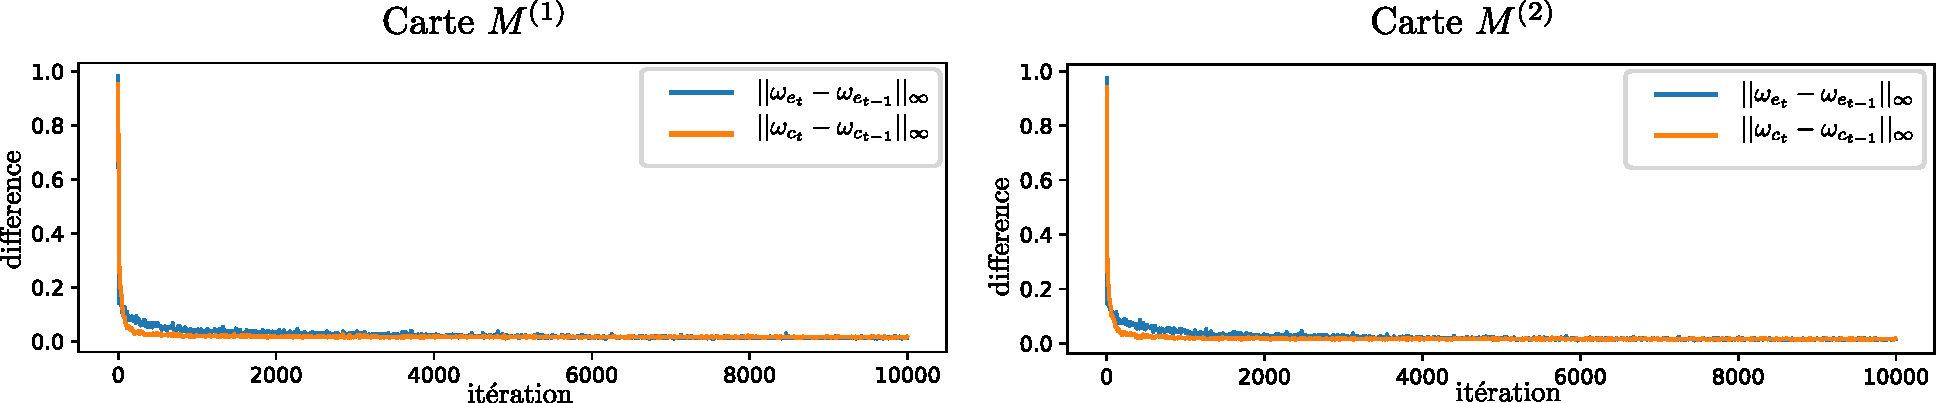
\includegraphics[width=\textwidth]{convergence/cercle_moy.pdf}
	\caption{Pour chaque carte, nous représentons l'évolution en fonction du temps d'apprentissage, de la différence maximale en valeur absolue entre les poids à l'instant $t$ et ceux à $t-1$ $\w_t$ et $\w_{t-1}$. Les entrées sont ici un cercle en deux dimensions. L'évolution est moyennée sur 10 apprentissages dont les entrées sont tirées aléatoirement selon la même distribution (cercle)
	Ces tracés montrent que les poids externes et contextuels convergent rapidement vers une position stable.\label{fig:conv}}
\end{figure}


\subsubsection{Disposition des poids}

Analysons maintenant la forme des poids contextuels de $M\m{1}$, tracés en figure~\ref{fig:w}.
Les poids externes, en orange, présentent une disposition similaire à ceux observés dans une carte classique. Les poids contextuels, en bleu, présentent une forme de vagues. Nous ajoutons à ces deux courbes le tracé des valeurs des entrées selon la position de leur BMU, en vert et rose sur la figure.

On remarque d'abord que les positions dans la carte $M\m{1}$ se répartissent en zones de BMUs, séparées par des zones mortes dans lesquelles aucune entrée n'a gagné. 
C'est une première différence avec une carte classique, pour laquelle toutes les positions seront BMUs lorsque les entrées sont distribuées de façon continue.
Les zones dans lesquelles il y a des BMUs correspondent aux extremum des poids contextuels et leurs alentours.

Dans la carte $M\m{1}$, les entrées externes $\inpx\m{1}$ sont proches de la courbe de poids externes, mais avec plus d'erreur de quantification que ce qu'on attendrait dans une carte simple. Une quantification vectorielle correcte est souhaitable, car elle permet de lier de retrouver la valeur de l'entrée à partir de la réponse d'une carte.
Nous notons que les zones définies par les poids contextuels partagent les positions des BMUs en fonction de la valeur des entrées. 
Deux points ayant la même valeur de $\inpx\m{1}$ mais une valeur différente de $\inpx\m{2}$ auront BMU différent dans la carte $M\m{1}$~; ces BMUs sont alors situées dans deux zones adjacentes.

Ainsi, une carte connectée au sein d'une architecture CxSOM différencie les échantillons en fonction de non seulement leur entrée externe, mais aussi de l'entrée de l'autre carte de l'architecture. La plage de valeurs des $\inpx\m{1}$ gagnant dans un des zones recoupe les plages de valeurs gagnant dans les zones situées à gauche et à droite. Par exemple, la zone dans laquelle l'échantillon rouge gagne, autour de $\bmu\m{1} = 0.25$. La partie des entrées située en dessous de la courbe de poids externe recoupe les valeurs d'entrées gagnant dans la zone précédente; la partie située au dessous de la courbe de poids externe recoupe des valeurs gagnant dans la partie suivante. Pour une entrée externe, le choix de la zone de BMU dans laquelle elle gagnera dépend alors de l'entrée contextuelle. 


Dans la carte $M\m{1}$, une position se spécialise donc en tant que BMU par rapport aux deux entrées et non pas une seule comme dans la carte indépendante~: les entrées externes et l'entrée contextuelles. C'est bien ce à quoi on s'attendait en ayant deux couches de poids. Ce qui est intéressant est que cette différenciation est réalisée par la répartition des unités en un nombre fini de zones distinctes. Dans chaque zone, les unités sont BMUs pour un segment de valeurs d'entrée externe et contextuelles. Au sein d'une zone, la répartition des entrées externe selon le BMUs est ordonnée, comme ce serait le cas dans une carte auto-organisatrice classique. Le comportement de la carte au sein d'une zone reste donc similaire à celui d'une carte classique.

Deux zones adjacentes correspondent par ailleurs à des segments de valeur d'entrée en partie superposés, et des segments de valeurs d'entrées contextuelles différentes. Il s'agit d'une deuxième échelle d'organisation, qui garde également l'aspect ordonné d'une carte classique. Ces zones sont créées par auto-organisation~; aucun paramètre de la carte n'a été modifié pendant l'apprentissage pour former ces zones, et le nombre d'unités allouées par auto-organisation dans chaque zone est à peu près égal. La carte agit un peu comme une base de données structurée avec des indices primaires et des indices secondaires pour chaque neurone, l'indice primaire étant la zone de la carte, et l'indice secondaire la position dans cette zone.

\begin{figure}
	\centering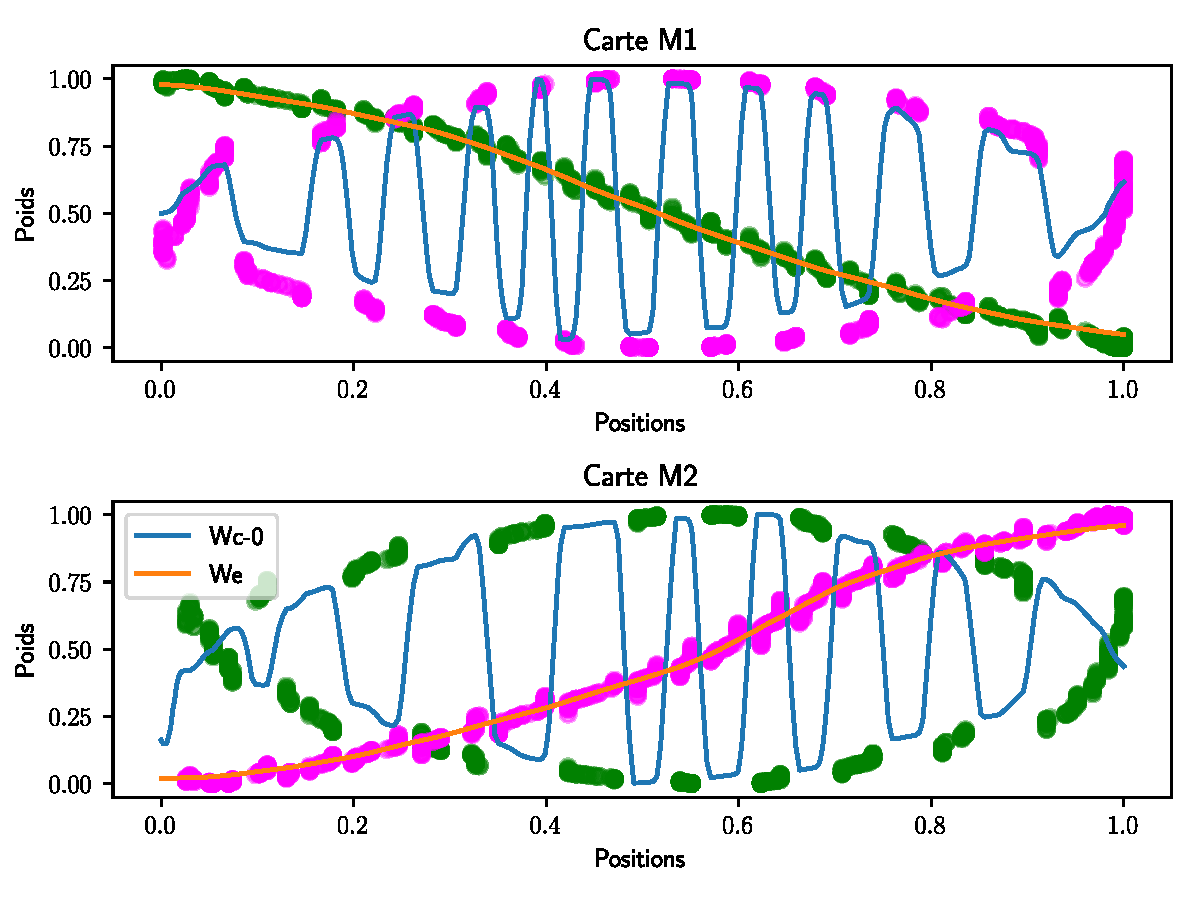
\includegraphics[width=0.9\textwidth]{2som_cercle_w.pdf}
	\caption{Représentation cartographique des poids et entrées lors d'une phase de test selon la position dans chacune des cartes. Nous remarquons que les poids d'une carte, par exemple la carte $M^{(1)}$ s'organisent en zones différenciant les valeurs de la paire $X^{(1)}, X^{(2)}$ et non seulement de la valeur de $X^{(1)}$. Deux zones adjacentes codent pour des valeurs de $X^{(1)}$ proches, mais $X^{(2)}$ différents. Au sein d'une même zone, les BMUs s'organisent sous la forme d'une sous-carte auto-organisée sur les valeurs de l'entrée contextuelle. Ces zones se forment de manière auto-organisée. \label{fig:w}}
\end{figure}

\begin{figure}
	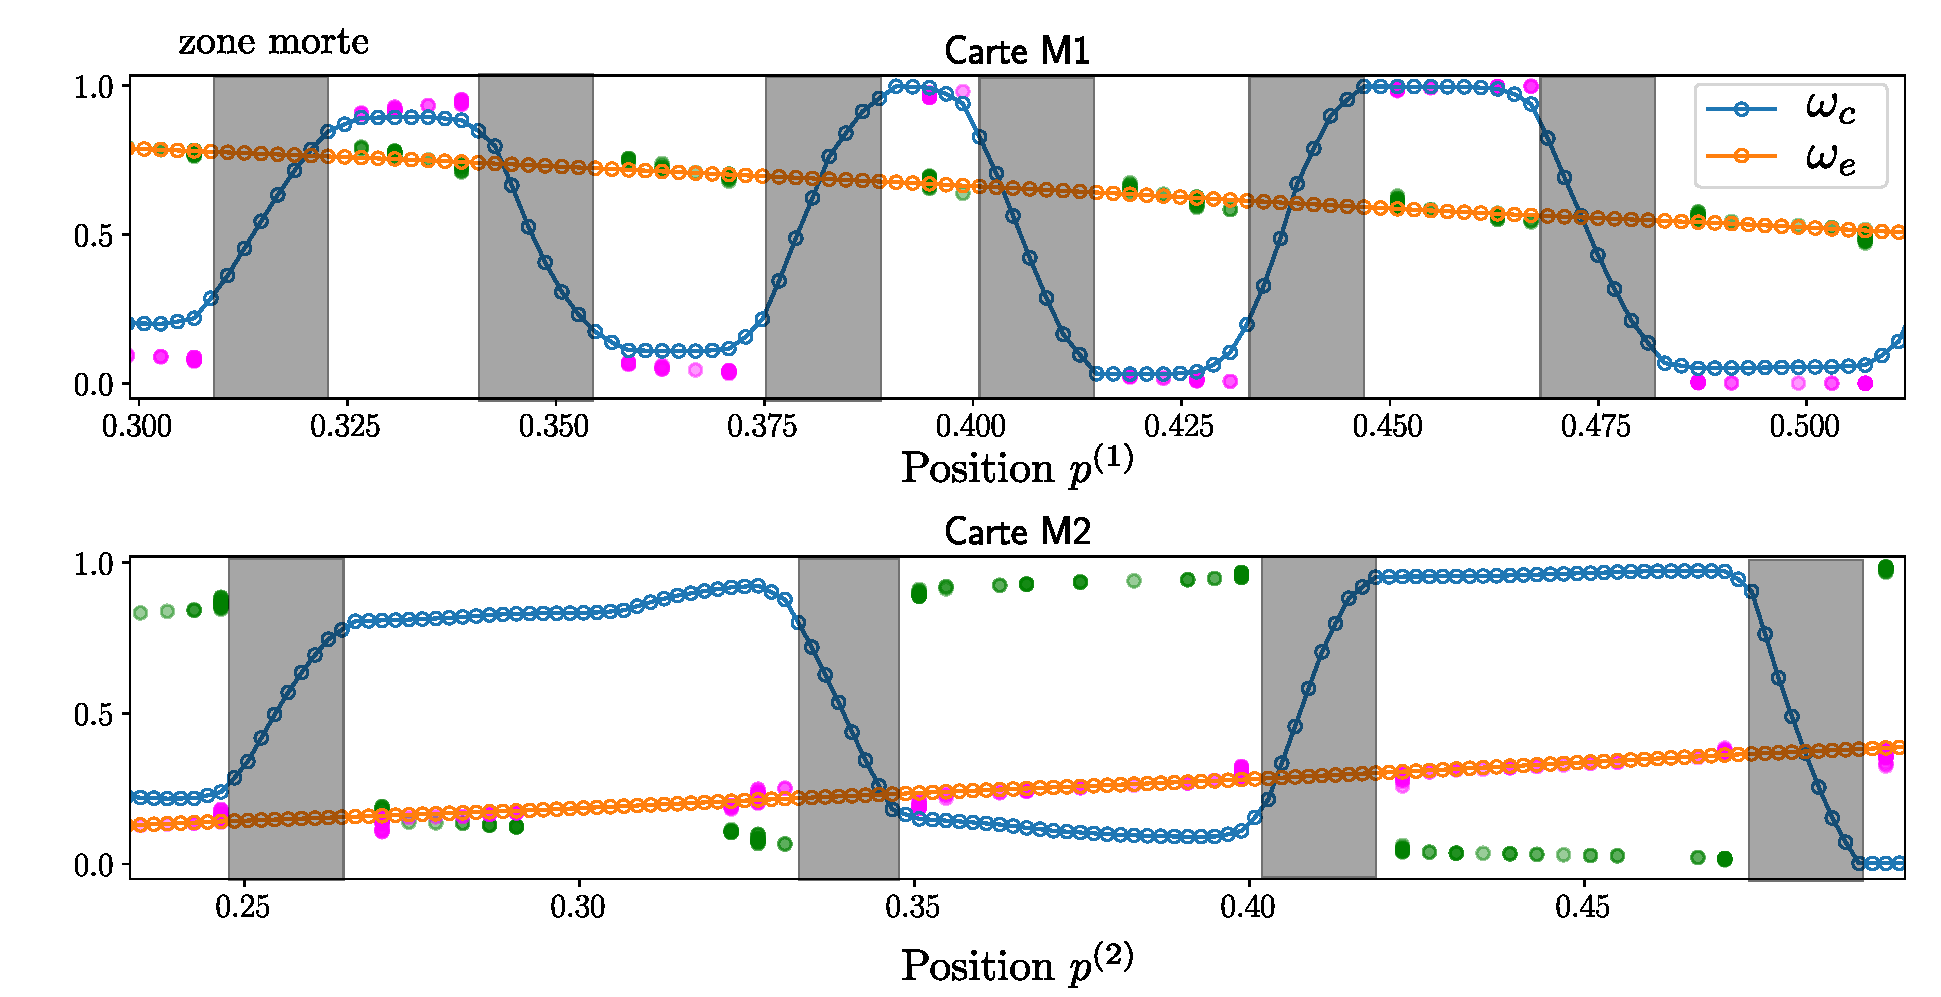
\includegraphics[width=\textwidth]{2som_cercle_w_zoom_with_nodes.pdf}
	\caption{Zoom sur la figure \ref{fig:w}. Nous y faisons apparaître la position sur la courbe des noeuds de la carte. Nous voyons que les zones grisées contiennent quelques n\oe{}uds qui ne sont jamais BMUsé; ce sont des zones mortes. Nous en concluons que la discontinuité introduite par la formation de zones est une "fausse" discontinuité et se produit en reliant des valeur de $\w_c$ éloignée en étirant une portion de carte morte. \label{fig:w_zoom}}
\end{figure}


\subsubsection{Erreur de quantification vectorielle}

La Figure~\ref{fig:qv} présente la valeur de l'entrée quantifiée au sein de chaque carte $\w\ext(\bmu\m{i})$ en fonction de l'entrée présentée $\inpx\m{i}$. Nous pouvons observer que la quantification vectorielle est bien réalisée. Cette capacité de quantification permet de retrouver la valeur de l'entrée à partir du BMU de la carte et donne donc une sortie interprétable dans l'espace des entrées à l'architecture CxSOM.
Cependant, l'erreur de quantification est plus forte que ce qu'on peut attendre avec une carte de même taille et mêmes paramètres apprenant sur l'ensemble de $\inpx\m{i}$. Nous remarquons une disposition en étages, dues aux zones formées par les poids contextuels.
Les n\oe{}uds de zones adjacentes de la carte sont en effet des Best Matching Unit pour des intervalles d'entrée qui se recoupent, ce qu'on observe sur la quantification vectorielle. Cependant, les poids externes restent croissants même entre deux zones, d'où la perte de précision. 

\begin{figure}
	\centering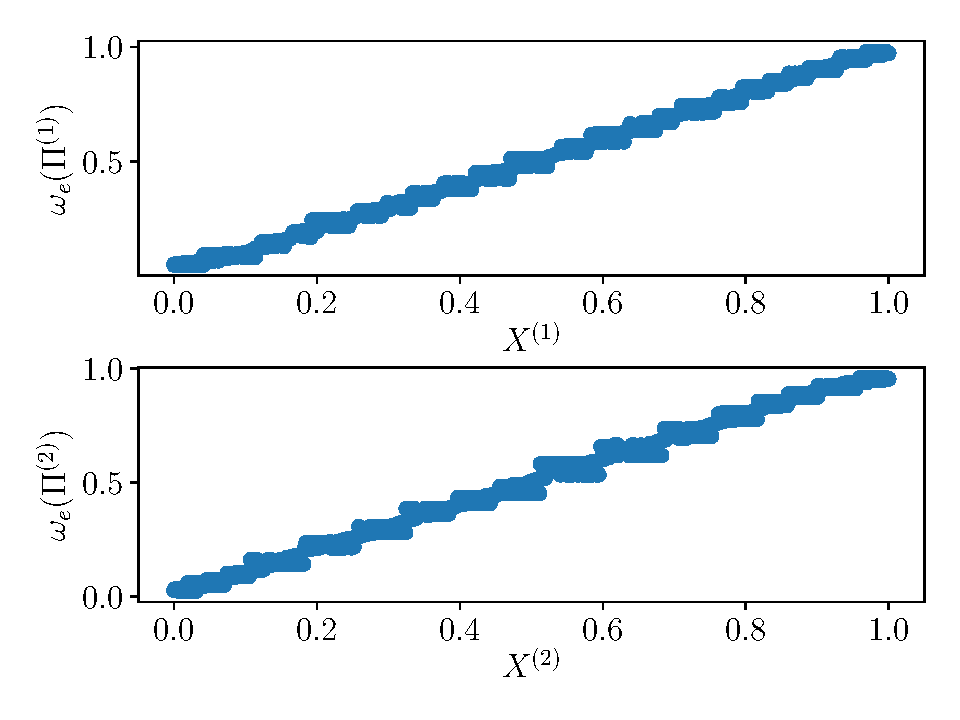
\includegraphics[width=0.8\textwidth]{2som_cercle_err.pdf}
	\caption{Représentation de l'erreur de quantification sur les valeurs de $X^{(1)}$ et $X^{(2)}$. Le poids externe du BMU est proche de la valeur de l'entrée~; chaque carte réalise ainsi une bonne quantification vectorielle sur ses entrées. \label{fig:qv}}
\end{figure}

\subsubsection{Conclusion}

Les résultats de cette expérience nous permettent donc de formuler les hypothèses suivantes concernant le comportement de cartes en une dimension~:

\begin{itemize}
	\item Chaque carte de l'architecture présente une faible erreur de quantification vectorielle sur ses entrées externes \ref{fig:qv}
	\item Les poids contextuels de chaque carte s'organisent en zones distinctes. Une zone correspond à un même intervalle de valeur pour $\inpx$ et $U$. Deux zones adjacentes encodent le même intervalle de valeurs pour $X$ mais des valeurs distinctes de $U$. \ref{fig:w} Ces zones se caractérisent par un étirement de la carte entre deux valeurs éloignées, apportant un aspect discontinu. Cette discontinuité passe en fait par la présence d'une zone peu dense de la carte contenant des n\oe{}uds qui ne seront jamais BMUs \ref{fig:w_zoom}. Nous verrons en section Prédiction que la formation de ces zones permet à la carte de prendre des décisions lors d'une phase de prédiction d'entrée.
	\item L'apprentissage du modèle d'entrée par l'architecture se traduit par l'existence d'une relation fonctionnelle entre $U$ et $\bmu$ dans chaque carte, montrant que chaque carte encode l'état de toute l'architecture et non seulement des entrées externes.
\end{itemize}

Nous chercherons à vérifier toutes ces observations sur d'autres dispositions d'entrées dans des structures de deux cartes, et nous nous demanderons si la création de zones dépend de la disposition des entrées. Nous chercherons donc à savoir comment ces zones sont construites. Enfin, une caractéristique d'une carte de Kohonen est sa robustesse au bruit. Nous vérifierons si cette propriété se traduit également dans les architectures de deux cartes.
Nous étendrons ensuite notre étude aux structures de trois cartes apprenant sur trois entrées 1D en section~\ref{sec:pred}.


%2SOM anneau ???


% \begin{figure}
% 	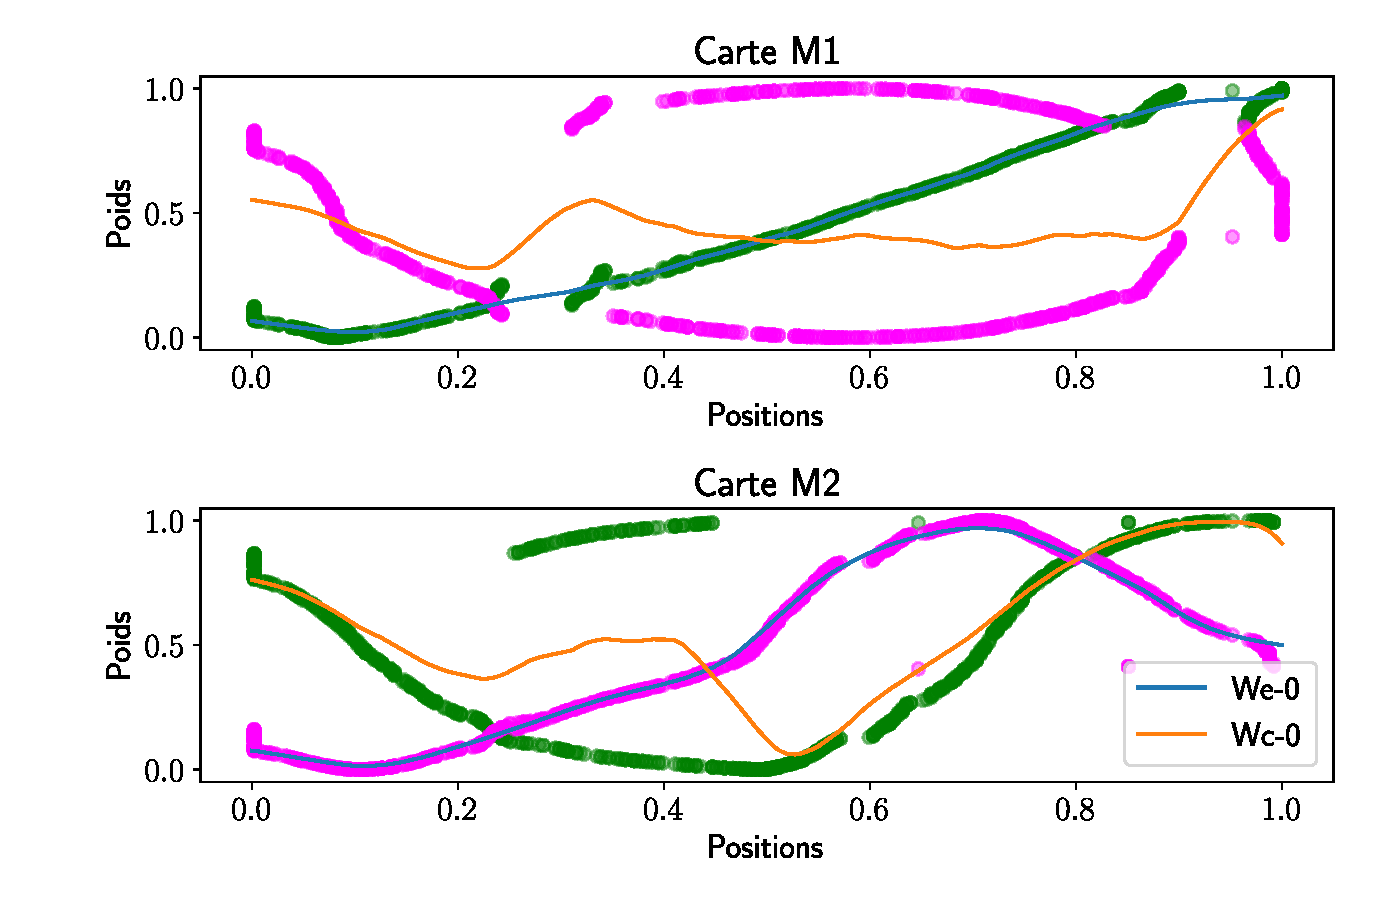
\includegraphics[width=\textwidth]{weights_rcre.pdf}
% 	\caption{Représentation cartographique des poids de la carte lorsque $r_c = r_e = 0.1$. La présence de zones n'est pas observée.}
% \end{figure}

\subsection{Vérification des hypothèses sur différentes distributions d'entrées}

La figure \ref{fig:id_results} présente la disposition des poids et entrées des cartes lorsque $\inpx\m{1}$ et $\inpx\m{2}$ sont identiques. Les poids externes et contextuels ne forment pas de zones et les deux cartes se comportent comme une seule carte simple sur $\inpx\m{1} = \inpx\m{2}$.
En figure~\ref{fig:cos_results}, la dépendance entre les entrées n'est plus bijective. $\inpx\m{2}$ est fonction de $\inpx\m{1}$~; de ce fait, la carte $M\m{1}$ ne forme pas de zones. Au contraire, la carte $M\m{2}$ doit a présent se diviser pour apprendre les deux valeurs de $\bmu\m{1}$ possibles correspondant à $\inpx\m{2}$. Ces expériences montrent que la formation de zones est relative à la disposition des entrées.

\begin{figure}
	\centering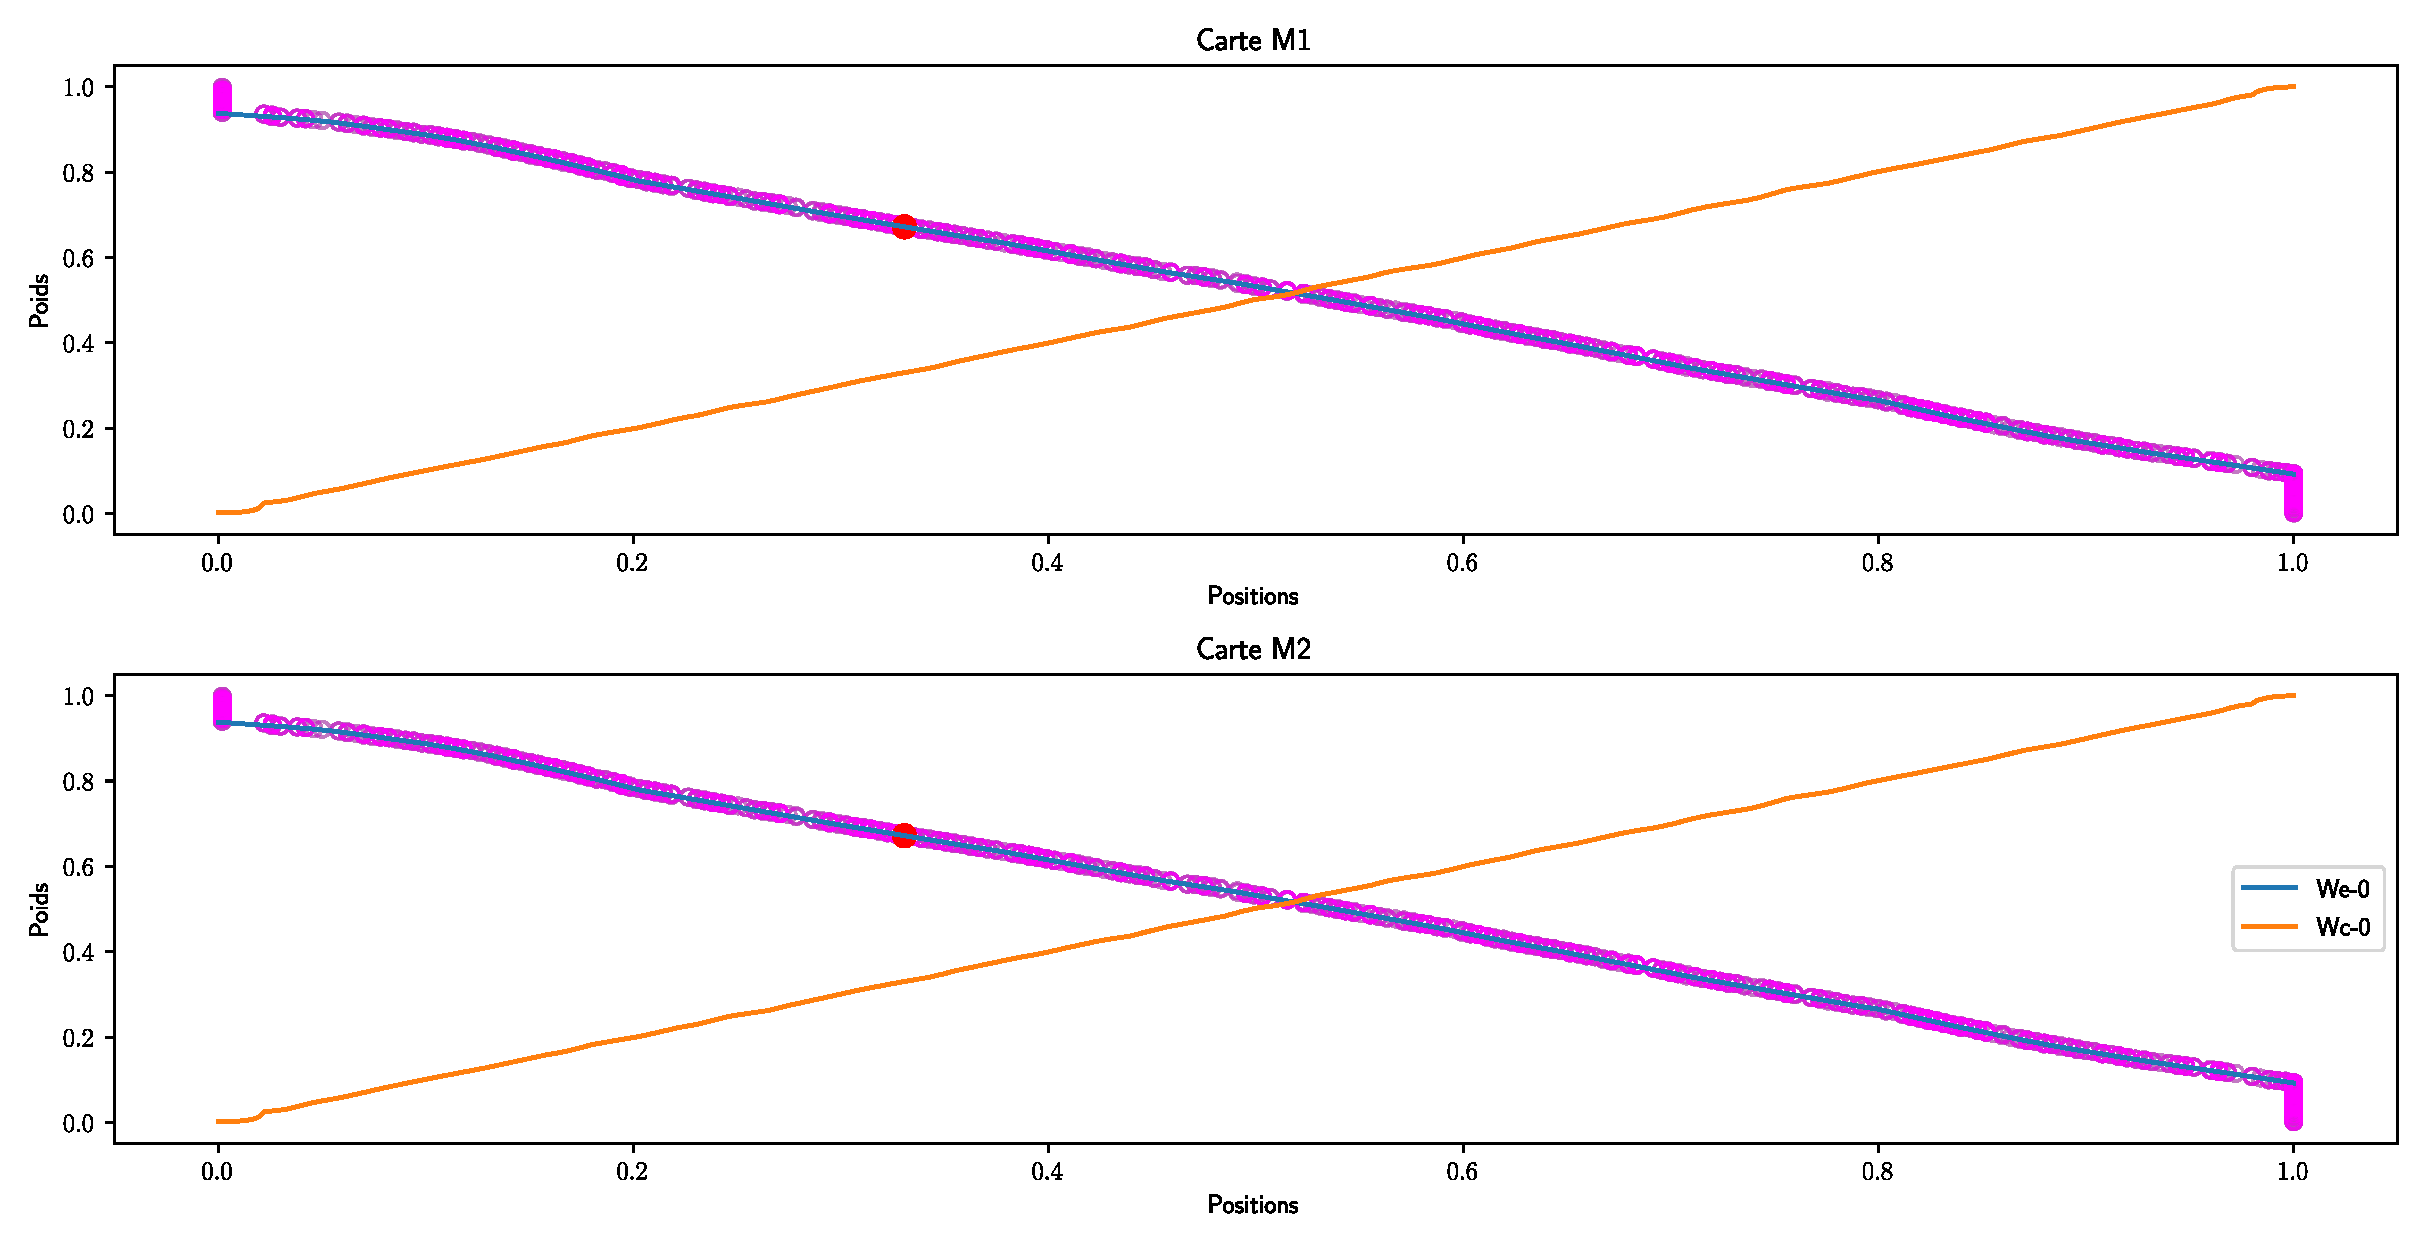
\includegraphics[width=0.6\textwidth]{2som_id_w.pdf}
	\caption{Représentation cartographique des poids et entrées pour la disposition identité. Les poids externes et contextuels sont superposés, et les poids contextuels n'ont pas besoin de former de zones \label{fig:id_results}}
	\end{figure}
	
	\begin{figure}
		\centering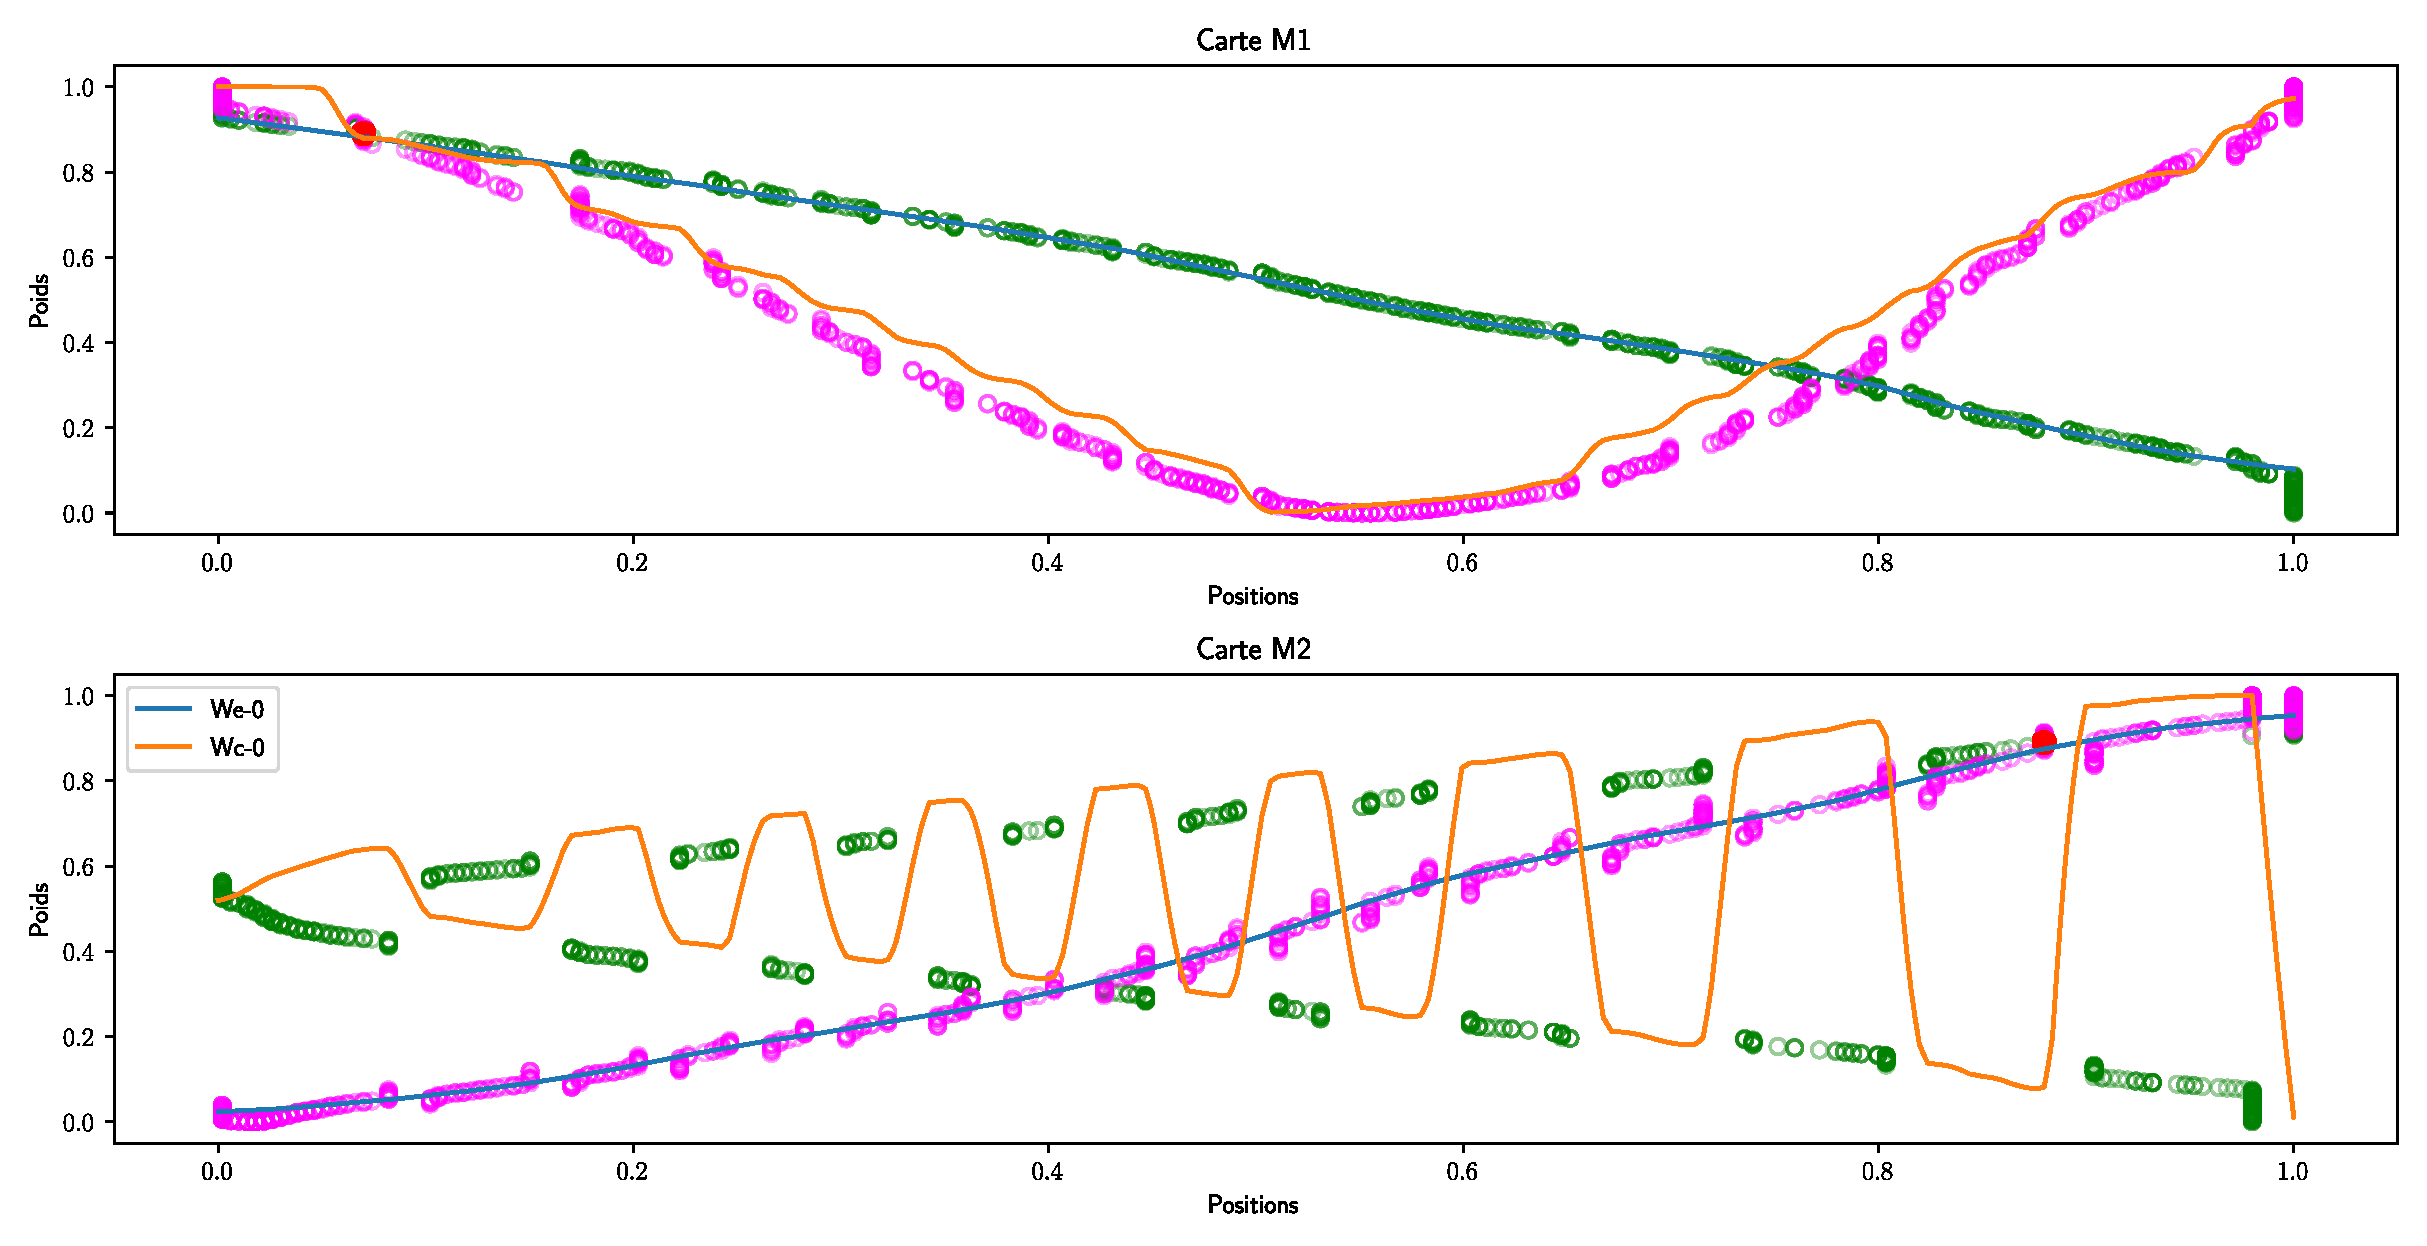
\includegraphics[width=0.7\textwidth]{2som_cos_w.pdf}
		\caption{Représentation cartographique des poids et entrées pour $\inpx\m{2} = cos(\inpx\m{1}$. Les poids contextuels de la carte $M\m{1}$ ne forment pas de zones car une seule valeur de $\inpx\m{2}$ correspond à une entrée $\inpx\m{1}$. Au contraire, les poids de la carte $M\m{2}$ s'organisent pour gérer la distinction. \label{fig:cos_results}}
	\end{figure}

La couche de poids externe converge plus vite que la couche contextuelle par la différence entre rayons de voisinage. De ce fait, les positions du BMU respectent les relations de distances dans l'espace d'entrée externe~: deux points éloignés sur $\w_e$ ont des poids éloignés.

Dans l'exemple du cercle, une valeur de $\inpx\m{1}$ correspond à exactement deux valeurs de $\inpx\m{2}$. Il est plus intéressant d'étudier l'organisation des cartes lorsque le nombre de valeurs possibles pour $\inpx\m{2}$ pour une même valeur de $\inpx\m{1}$ augmente. On peut supposer que la carte continuera à s'organiser en zones. 
Il faudrait cependant un nombre bien plus élevé de zones dans une carte pour gérer exhaustivement toutes les configurations d'entrées possibles.
Nous traçons en Figure~\ref{fig:lissa} l'organisation obtenue pour des points placés sur une courbe de Lissajous, dans laquelle une valeur de $X\m{1}$ correspond à 4 à 6 valeurs de $\inpx\m{2}$ et inversement. 
Enfin, la figure~\ref{fig:ind} présente l'organisation obtenue lorsque les points sont dans le carré $[0,1]^2$~: les entrées sont indépendantes, une valeur de $\inpx\m{1}$ correspond à une infinité de valeurs pour $\inpx\m{2}$. 

Dans ces deux derniers cas, les cartes présentent une organisation en zones des poids contextuels, tout comme le comportement observé sur le cercle. Le nombre et la forme des zones est similaire à celle du cercle au niveau des poids contextuels~: nous n'observons pas de zones dans les zones. Cependant, contrairement au cercle, les BMUs se répartissent sur toutes les valeurs de $\w_c$ dans une zone.
Ainsi, nous pouvons conclure que la présence de zones en tant que telle est donc un comportement systématique de la carte étant donné qu'elles sont observées même lorsque les entrées sont indépendantes. Par contre, la forme des zones dépend de la relation entre entrée.
Sur la distribution indépendante, contrairement au cercle, la carte ne présente pas de zone morte. La totalité d'une zone se déploie de manière à couvrir l'ensemble des valeurs de $U$, ce qui est également observé en figure ~\ref{fig:lissa} pour les courbes de Lissajous.
Une zone agit alors comme une petite carte d'une sous-région de l'espace d'entrée. Nous pouvons le constater sur la Figure~\ref{fig:2som_p_d} présentant la distorsion des poids externes des cartes dans l'espace $\inpx\m{1}; \inpx\m{2}$.


Nous avons remarqué que les poids externes se déplient en priorité. Ils respectent les distances~: deux n\oe{}uds distants dans la carte ont des poids distants et gagnent pour des entrées distantes.  
Par contre, deux n\oe{}uds proches peuvent gagner pour une même valeur d'entrée externe, bien qu'ayant une valeur de poids contextuel légèrement différente.
L'intervalle de valeurs d'entrées codées au sein de deux zones adjacentes se recouvrent.
Les deux cartes de Kohonen se comportent donc pour paver l'espace d'entrée différemment, et définissent un compromis entre qualité de l'approximation de l'entrée externe par $\w_e(\bmu)$ et différenciation des BMUs selon le modèle d'entrée complet $U$.


\begin{figure}
	\centering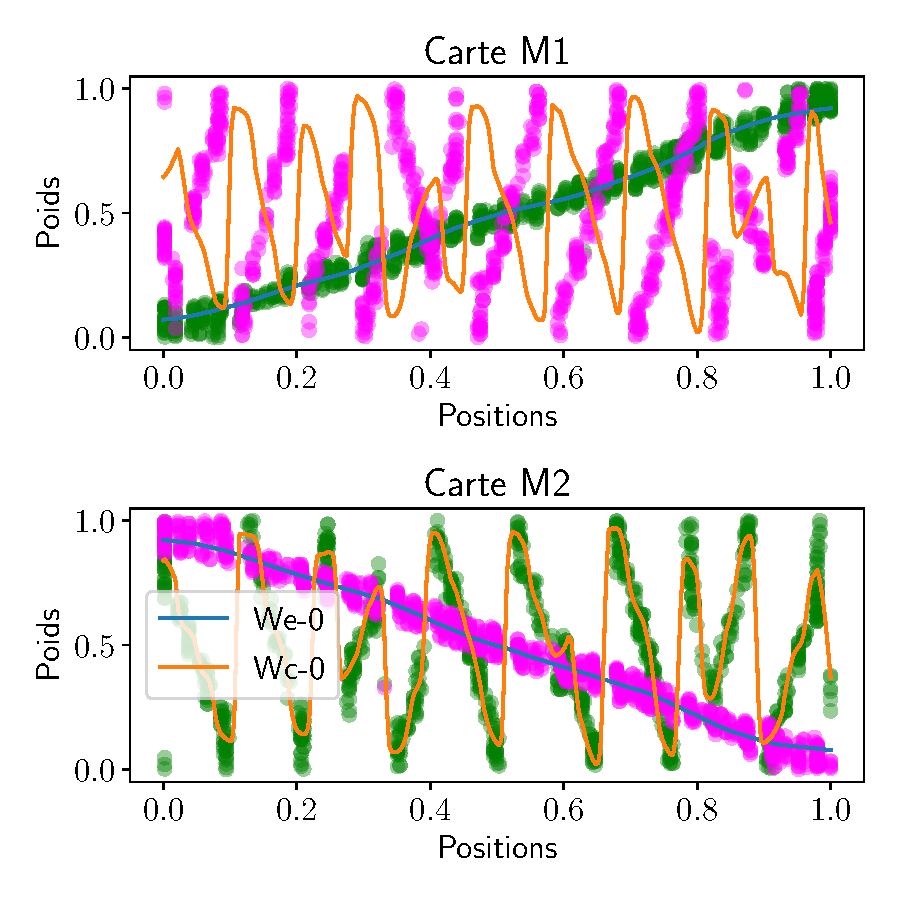
\includegraphics[width=0.6\textwidth]{2som_square_w.pdf}
	\caption{Représentation cartographique des poids et entrées pour la disposition carré}
\end{figure}

\begin{figure}
	\centering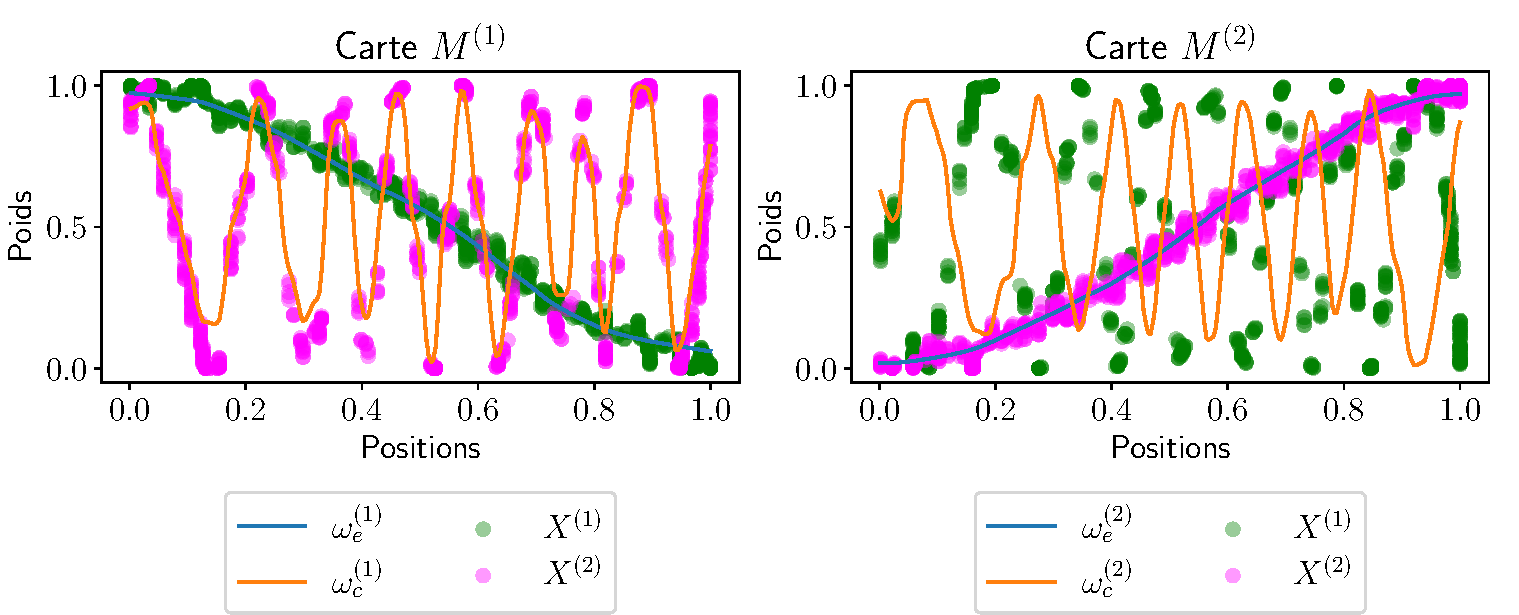
\includegraphics[width=0.6\textwidth]{lissa/weights_19999.pdf}
	\caption{Représentation cartographique des poids et entrées pour des entrées sur une courbe de Lissajous. Les poids contextuels continuent de former des zones.}
\end{figure}

\begin{figure}
	\begin{minipage}{0.48\textwidth}
		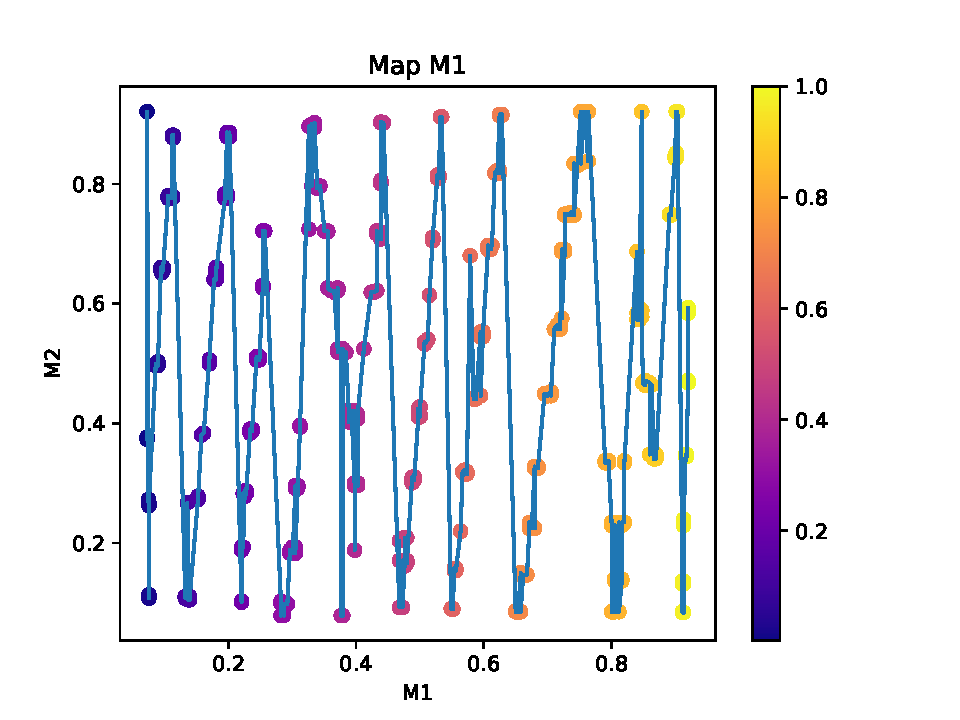
\includegraphics[width=\textwidth]{2som_square_d}
	\end{minipage}
	\begin{minipage}{0.48\textwidth}
		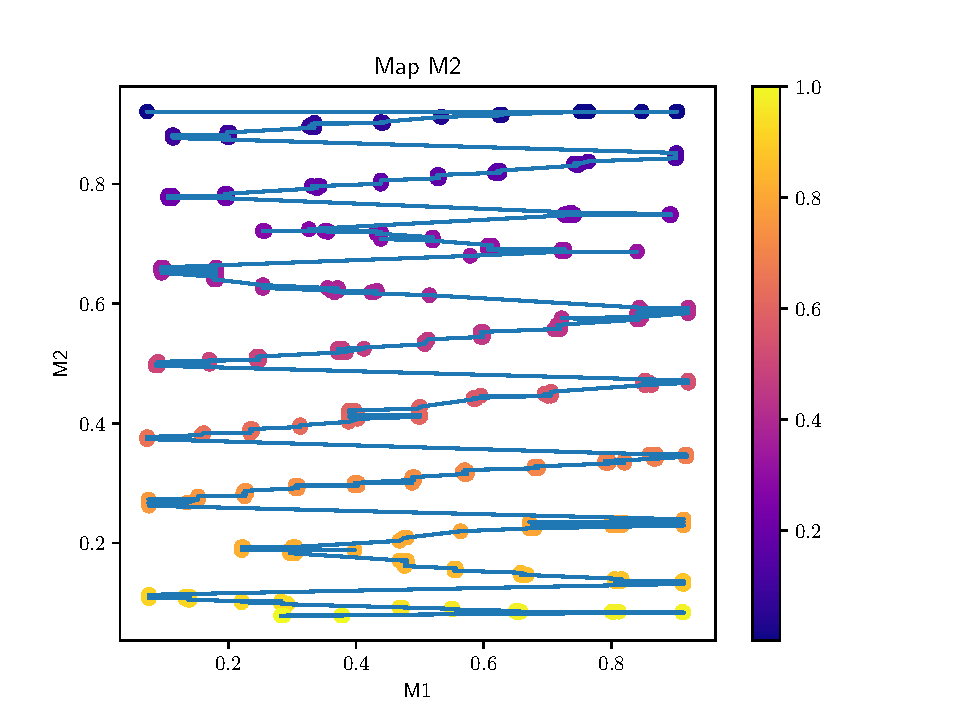
\includegraphics[width=\textwidth]{2som_square_d2}
	\end{minipage}
	\caption{Représentation de la distortion des poids des deux cartes dans l'espace d'entrée $\inpx\m{1}, \inpx\m{2}$ lorsque les entrées sont indépendantes. Les cartes s'organisent de façon à quadriller le carré, l'une selon les $\inpx\m{1}$, l'autre selon les $\inpx\m{2}$. Bien que chaque carte aie 500 noeuds, on observe seulement environ 90 valeurs possibles pour les paires $\w_e(\bmu\m{1}),\w_e(\bmu\m{2})$ \label{2som_p_d}}
\end{figure}



\subsection{Discussion}

Nous avons observé sur ces distributions d'entrées en 2D les comportements suivants qui vérifient et complètent les hypothèses formulées sur la disposition d'entrées en cercle.
La quantification vectorielle reste correctement réalisées sur les différentes dispositions d'entrées. Les valeurs prises par les poids sont toujours disposées en étages à cause des zones.
Cette organisation en zones intervient dès que la disposition des entrées implique d'avoir à séparer au moins deux valeurs de $U$ pour une même entrée externe. Le fait que des zones existent n'implique pas la détection d'une relation entre entrées mais est systémique aux mécanismes d'auto-organisation des cartes. Par contre, l'organisation au sein d'une zone et forme des poids contextuels dépend de la dépendance entre les entrées.


La disposition des cartes repose ainsi complètement sur les zones formées par les poids contextuels. Ces zones apparaissent grâce au fait que la proximité des poids externe est priorisé par rapport au poids contextuels par le rayon de voisinage externe 10 fois plus élevé. Ce rapport introduit une relation subordonnée entre les poids. 
Ces zones semblent favoriser la recherche de consensus lors de la relaxation et la convergence des poids~; cet avantage n'est pas significativement observable en une dimension, dans laquelle les poids des cartes convergent très facilement.
Par contre, nous verrons en partie suivante que ces zones permettent à l'architecture d'utiliser une carte en tant que prédiction d'entrée, ce qui n'est pas possible lorsque les cartes ne sont pas organisées en zones.


Au sein d'une même zone, dans laquelle les poids externes ont des valeurs très proches, les poids contextuels s'organisent de manière à former une petite carte sur toutes les valeurs possible de l'entrée contextuelle.
On pourrait donc introduire une notion d'indices primaire et secondaire, l'indice primaire étant celui de la zone et l'indice secondaire la position dans la zone.
Cette notion d'indices primaires et secondaires est également observée dans le cerveau, proposé en 1986 par \cite{ballard_cortical_1986}. Les neurones du cortex V1, par exemple, gèrent leurs connexions et leur organisation comme schématisé en figure~\ref{fig:ballard}.
Les neurones situés à différents emplacements sur cortex V1 ne reçoivent pas la même partie de l'entrée visuelle. Ces entrées différenciées forment une indexation~\emph{primaire} de V1. Au sein d'une zone de même indice primaire, les neurones s'organisent de façon à représenter tous le sous-espace des entrée ayant été présenté à la zone. Cette sous-carte définit alors des indices secondaires.
Ici, la même entrée est certes présentée à toute la carte, mais les BMUs des zones réagissent à un sous-ensemble d'entrées externes définies par les poids contextuels.

Le comportement des cartes jointes introduit par ailleurs un phénomène de discontinuité dans les poids contextuels. Cette discontinuité est en fait une fausse discontinuité puisque des zones mortes comptant quelques n\oe{}uds séparent deux zones de poids contextuels.
On observe que plus on a de valeurs possibles pour $\inpx\m{2}$ pour une même valeur de $\inpx\m{1}$, moins on aura de n\oe{}uds morts dans les zones de discontinuité, comme le montre l'exemple du carré dans lequel il n'y a pas de n\oe{}uds morts entre zones.
Les zones sont à peu près réparties équitablement sur la carte.
La présence de zones auto-organisées permet aux cartes d'acquérir une capacité de prise de décision, que nous explorons dans la section suivante.
En effet, si une carte ne possède pas d'entrée externe, elle peut être activée par les connexions contextuelles et possède un BMU. Nous verrons que l'architecture CxSOM permet une prédiction correcte seulement si les cartes se sont organisées en zones.

Ces architectures de quelques cartes sont des architectures \emph{élémentaires}~: toute architecture comportant plus de cartes pourra être construite à partir de petits modules.

Pour des cartes en une dimension, les comportements d'organisation en zones et de convergences observés sont reproducibles sur de nombreuses dispositions d'entrées pour de nombreuses condition initiales de poids des cartes.


\begin{figure}
	\centering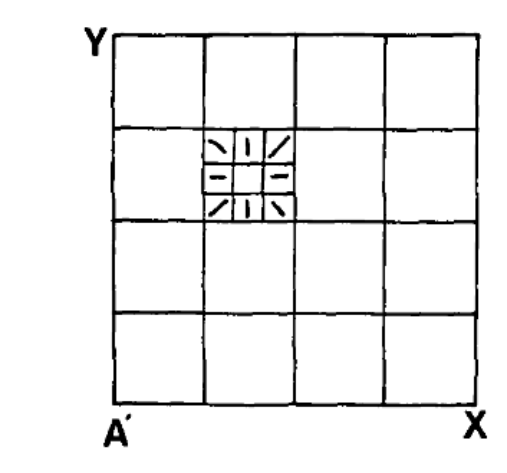
\includegraphics[width=0.5\textwidth]{ballard_primary_secondary.png}
	\caption{Schéma d'une répartition en indices primaires et secondaire des neurones d'une aire corticale présentée en \cite{ballard_cortical_1986}. Les auteurs observent que sur une carte rétinotopique des neurones, c'est à dire tracées en fonction de la position des neurones sur le cortex, la réponse de neurones est organisée en zones, les indices primaires, recevant en connexion différentes portions de l'espace d'entrée. Au sein d'une même zone, les neurones cartographient toutes les valeurs possibles de l'entrée sous forme de carte topologiquement ordonnée, formant des indices secondaires.\label{fig:ballard}}
\end{figure}

\subsection{Limites possibles et questions ouvertes}

- Influence des connexions contextuelles 
- Comparaison: carte en loop vs cartes connectées ,meme organisation des poids. prédiction réalisée, mais moins bonne. Les connexions distantes gardent donc bien une influence, sans quoi la prédiction n'est pas du tout possible, mais influence réduite.


- Paramètres : taille de la carte, dépendance de la taille de zone à rc, re


\begin{figure}
	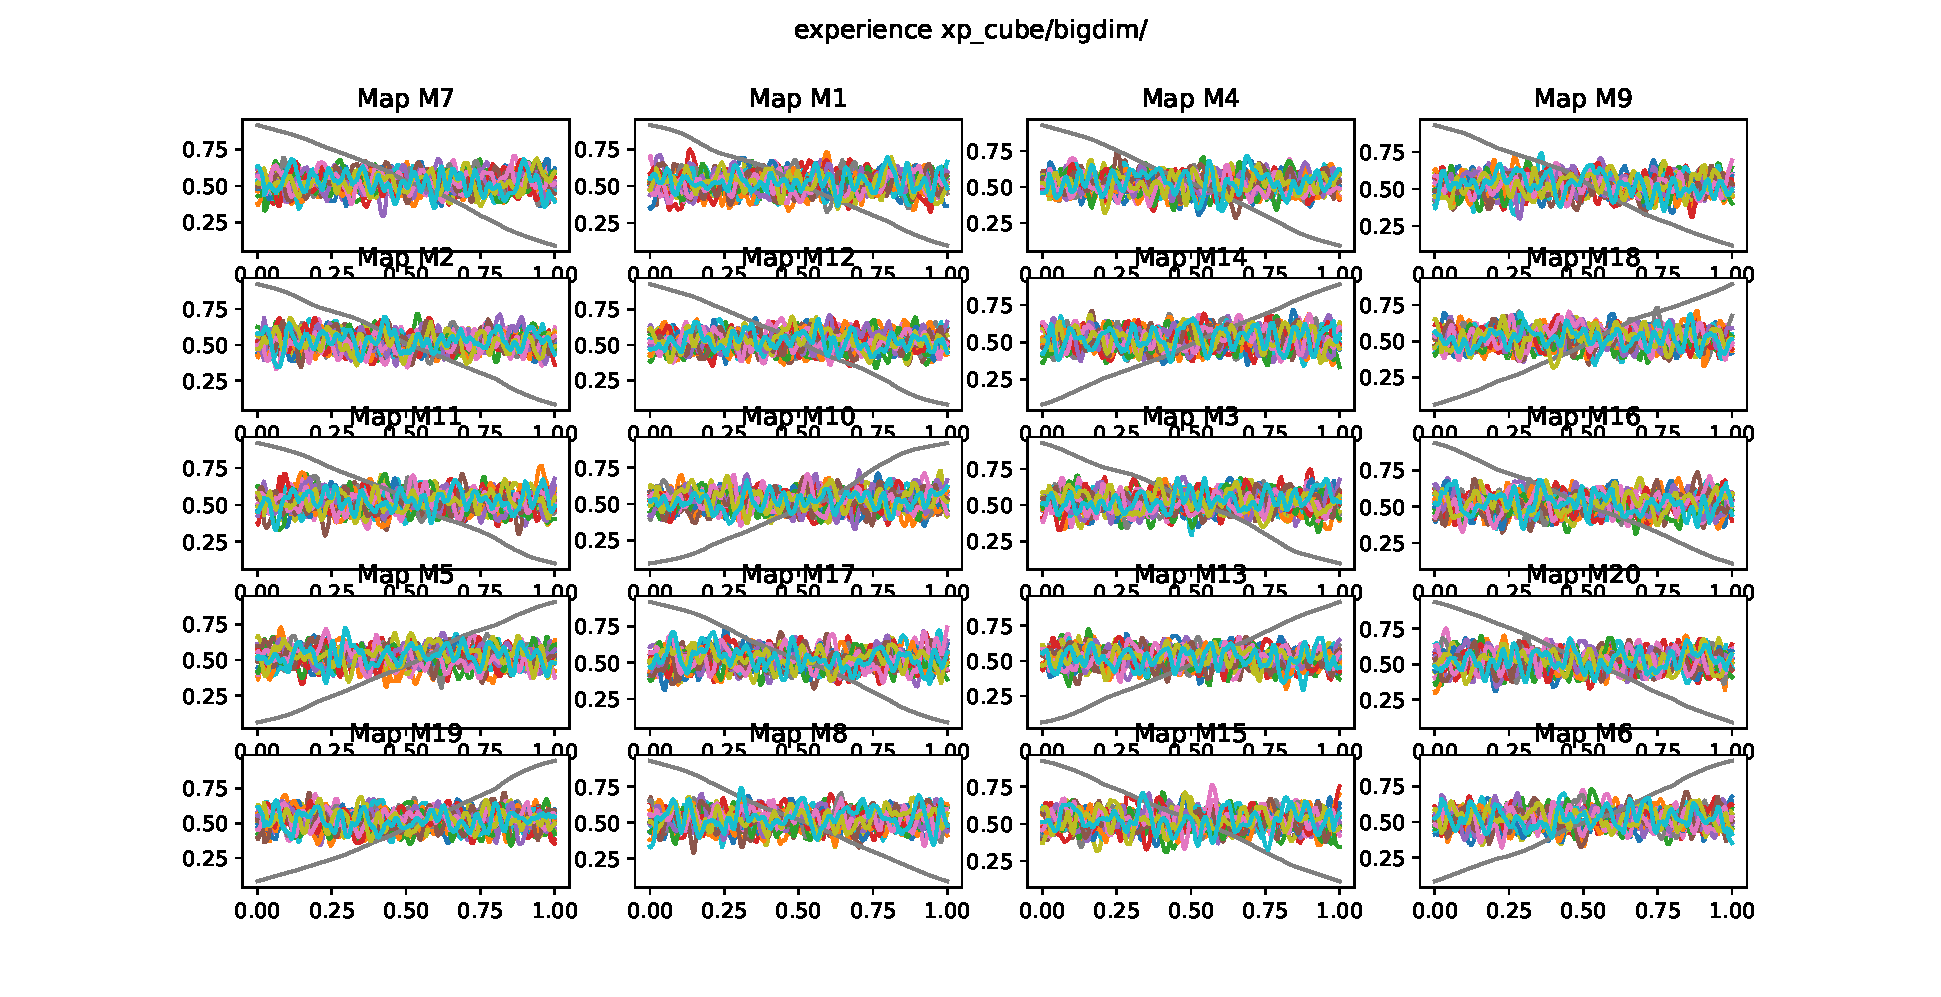
\includegraphics[width=\textwidth]{xp_cube_bigdim.pdf}
	\caption{Tracé des poids des cartes pour une architecture de 10 cartes toutes connectées. Les entrées sont ici indépendantes. Nous remarquons que les poids contextuels se moyennent autour de 0.5.}
\end{figure}

\begin{figure}
	\begin{minipage}{\textwidth}
		\centering\includegraphics[width=\textwidth]{loop/weights.pdf}
	\end{minipage}
	\begin{minipage}{\textwidth}
		\includegraphics[width=\textwidth]{loop/prediction.pdf}
		\caption{Poids à l'issue de l'apprentissage et erreur de prédiction de $\inpx\m{1}$ dans une architecture de 3 cartes connectées en boucle. Bien que les poids s'organisent de façon similaire aux expériences dans lesquelles les cartes sont connectées réciproquement, la prédiction est moins bien réalisée. L'influence des connexions diminue donc rapidement avec la distance dans l'architecture, mais reste présente.\label{fig:3som_loop}}
	\end{minipage}
\end{figure}

\section{Prédiction d'entrée}

L'observation des mécanismes d'organisation occurrant dans des architectures de deux cartes nous a confirmé que le modèle d'entrées, défini par la variable cachée, est appris dans chacune des cartes de l'architecture grâce aux connexions entre cartes.
Nous utilisons maintenant le fait qu'une architecture ait appris le modèle dans une tâche de prédiction d'entrée.

Cette utilisation en tant que prédiction a certes une valeur applicative, car il s'agit d'un cas d'utilisation possible d'une architecture CxSOM pour une tâche de mémoire associative. Néanmoins, la prédiction permet avant tout de valider l'apprentissage du modèle par l'architecture d'un point de vue d'une carte. Par exemple, dans le cas de données réelles, le modèle d'entrée n'est pas forcément connu. La prédiction permet alors de valider l'apprentissage du modèle.

La structure utilisée pour la tâche de prédiction est présentée en Figure~\ref{fig:schema_pred}. Dans un premier temps, les cartes CxSOM sont mises à jour sur l'ensemble des entrées dans une phase d'apprentissage. Ensuite, nous choisissons une des cartes comme carte prédictive. Lors de la phase de prédiction, cette carte ne reçoit plus d'entrée externe, mais seulement ses entrées contextuelles. 
Les autres cartes reçoivent quant à elles toujours leurs entrées externes et contextuelles. La phase de prédiction est une phase de test durant laquelle les poids de toutes les cartes ne sont pas mis à jour. Les règles de calcul et paramètres sont conservés entre apprentissage et prédiction.
La carte ne recevant pas d'entrée externe prend comme activité globale seulement son activité contextuelle.

Nous choisissons comme valeur de prédiction le poids externe du BMU de la carte prédictive $\w\ext\m{i}(\bmu\m{i})$. Ce BMU a été choisi uniquement grâce aux entrées contextuelles de la carte. Nous vérifierons alors que cette prédiction est proche de l'entrée théorique $\inpx\m{i}$ non présentée à la carte.

\begin{figure}
	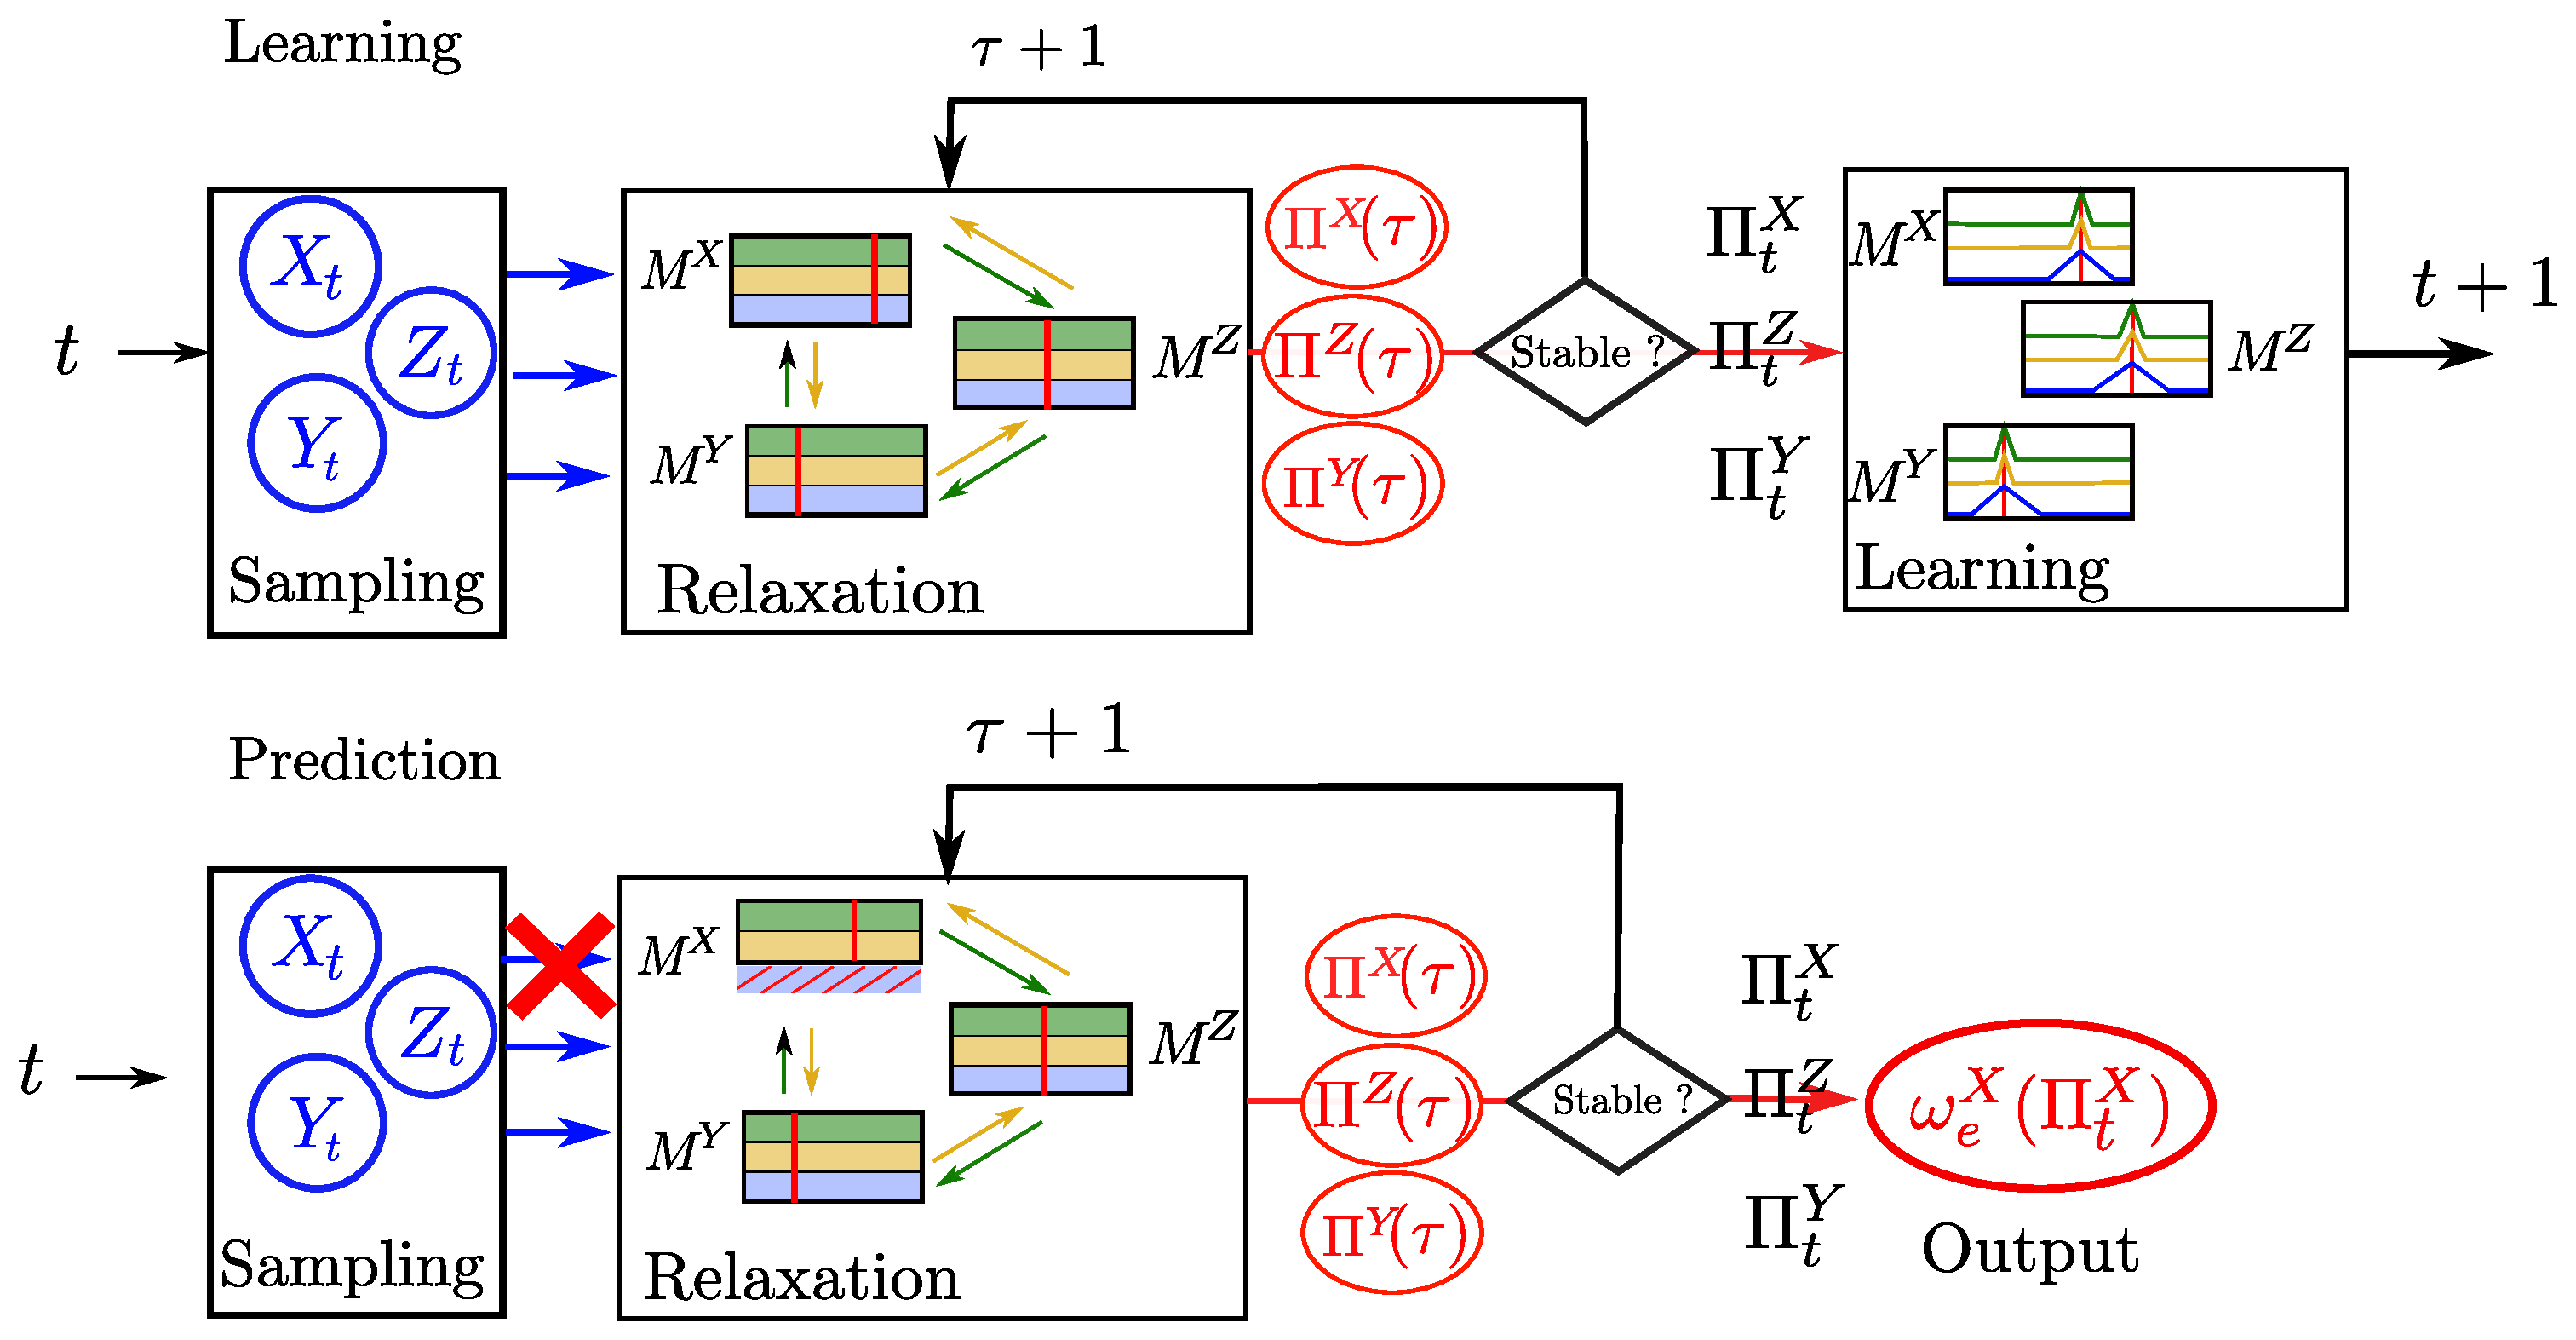
\includegraphics[width=\textwidth]{learning_tests.pdf}
	\caption{Schéma descriptif des opérations effectuées lors de l'apprentissage et de la phase de prédiction.\label{fig:schema_pred}}
\end{figure}

\subsection{Prédiction d'entrées géométriques}

Nous testons d'abord la qualité de la prédiction sur des dispositions d'entrées géométriques.
Pour qu'une carte puisse faire une prédiction correcte, nous choisissons des dispositions d'entrées telles que la connaissance des entrées et du modèle détermine l'entrée manquante.

Nous prendrons ainsi des entrées disposées sur un cercle en deux dimensions plongé et pivoté dans l'espace en 3D \ref{fig:cercle3}. De cette manière, la connaissance de deux des trois coordonnées permet de déterminer la troisième avec précision. Nous testerons également la prédiction d'entrée sur un plan 2D pivoté en trois dimensions.

Ces tâches de prédictions sont réalisées sur une architecture de trois cartes 1D, toutes connectées entre elles. Chaque carte prend donc deux entrées contextuelles et de ce fait possède deux couches contextuelles.
Nous étendrons la capacité de prédiction aux cartes deux dimensions au chapitre suivant.

\begin{figure}
	\centering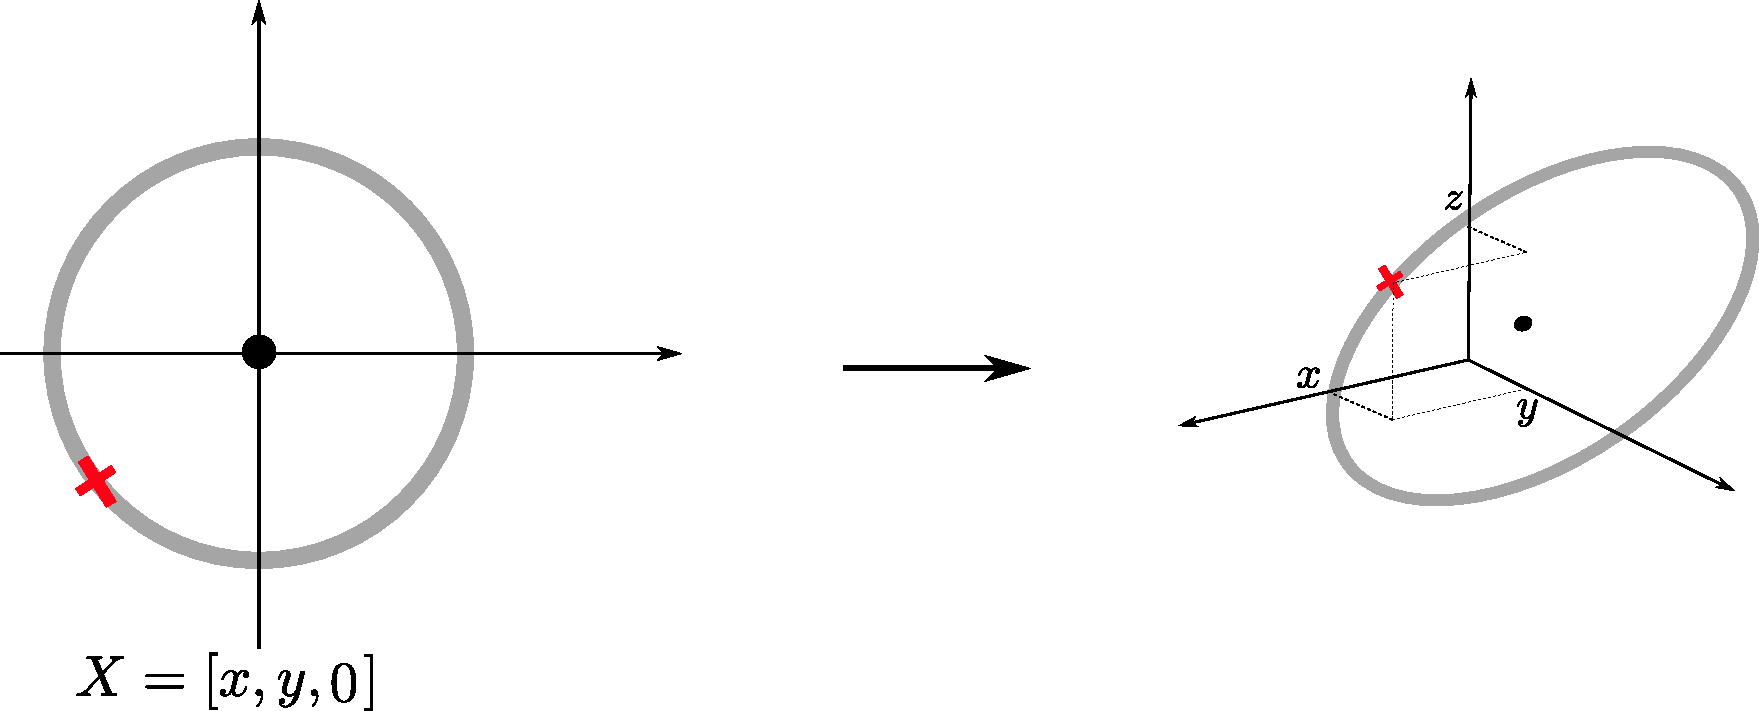
\includegraphics[width=0.9\textwidth]{anneau_inputs.pdf}
	\caption{Exemple de courbe plongée en trois dimensions. La figure 2D est pivotée en trois dimensions. Chaque coordonnée est normalisée de façon à s'étendre entre 0 et 1 en trois dimensions.
	\label{fig:in_3D}}
\end{figure}

La figure \ref{fig:w_cercle} présente la disposition des poids des trois cartes de l'architecture après apprentissage ainsi que des entrées associées. 
Comme dans la version à deux cartes, les poids contextuels s'organisent en plusieurs zones au sein desquelles la valeur de $U$ est située dans une même plage de valeur.
Les deux couches de poids contextuels forment les mêmes zones.
La figure \ref{fig:pred_cercle} présente ensuite l'erreur obtenue lors de la phase de prédiction. L'entrée $X\m{1}$ n'est ici pas présentée à la carte et sa valeur est prédite par $\w\ext\m{1}{\bmu\m{1}}$. 
Cette figure nous montre que la prédiction est correctement réalisée par l'architecture de cartes. Remarquons que la disposition de l'erreur en lignes horizontales correspond aux zones définies par les valeurs des poids contextuels d'une carte.

Nous traçons également en Figure~\ref{fig:plan3} la disposition des cartes et l'erreur de prédiction obtenue pour des entrées située sur un plan 2D de l'espace en trois dimensions. Ici encore, La connaissance de $X\m{2}$ et $X\m{3}$ définit bien une seule valeur possible de $X\m{1}$. La prédiction est bien réalisée, en remarquant une erreur assez élevée. 
Nous avons vu que les poids externes des cartes s'étalaient sur le plan en discrétisant l'espace en une centaine de points seulement, bien que chaque carte soit de taille 500 (Voir Figure~\ref{fig:2som_p_d}). 
Cette discrétisation se retrouve dans l'erreur de prédiction pour trois cartes.

Cette capacité de prédiction est peu précise, mais il s'agit d'une prise de décision induite par l'auto-organisation des cartes.
La formation de zones discrètes apparaît comme nécessaire à cette capacité prédictive. Par exemple, nous présentons en Figure~\ref{fig:rcre_pred} l'erreur de prédiction dans une architecture de 3 cartes sur un cercle 2D, mais dans lesquelles on a pris $r_c = r_e$. Ce jeu de paramètre ne fait pas apparaître de zones dans les poids contextuels. Nous voyons alors qu'aucune prédiction n'est réalisée. Dans ce sens, bien que les cartes se soit organisées, on ne peut pas parler d'un apprentissage du modèle par l'architecture.

Lorsqu'il manque des informations pour prédire correctement l'entrée, par exemple dans le cas du cercle en deux dimensions et d'une architecture de deux cartes, l'activation est cohérente. Si on ne présente pas l'entrée $\inpx\m{2}$ à la carte $M\m{2}$, deux bulles d'activité se formeront aux deux emplacements possibles pour $\bmu\m{2}$. D'après la figure~\ref{fig:pred_closed}, le choix de l'une ou l'autre des valeurs est aléatoire~: une des deux options n'est pas systématiquement privilégiée.


% La figure \ref{fig:w_lissa} présente la disposition des poids sur une courbe de lissajous.
\begin{figure}
	\centering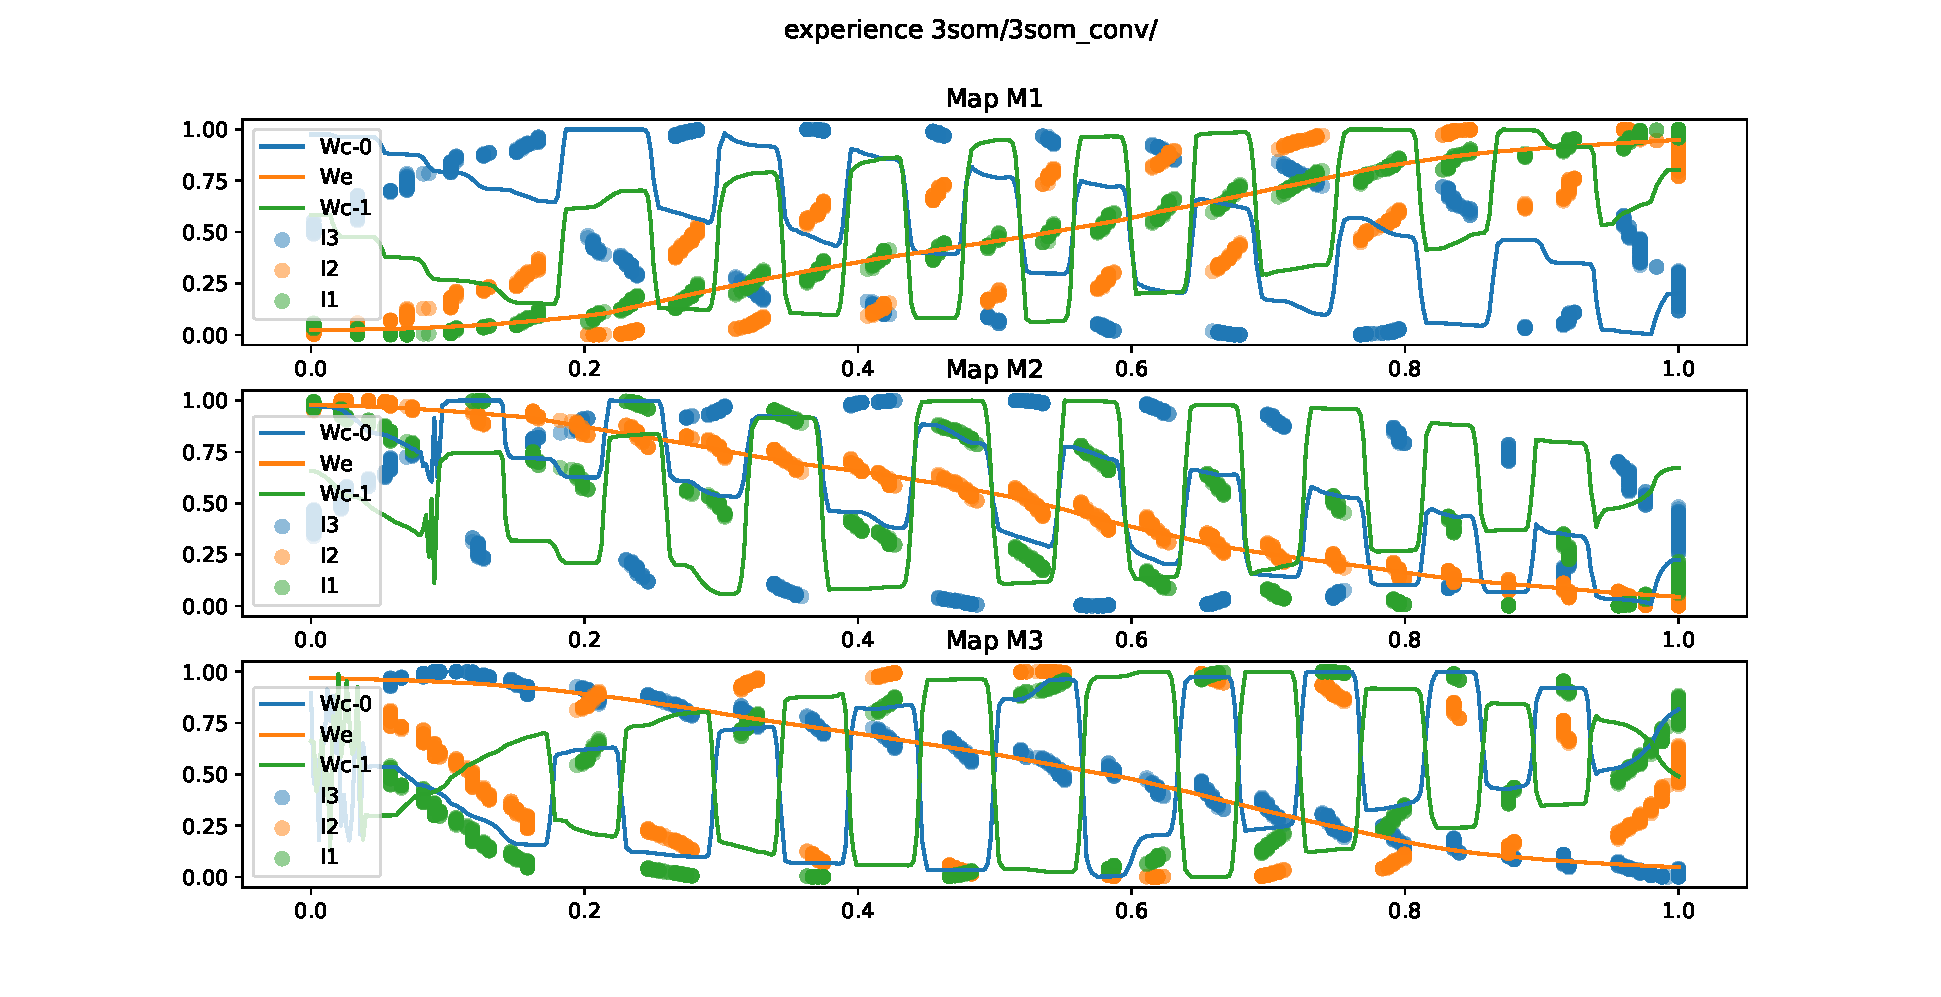
\includegraphics[width=0.9\textwidth]{3som_cercle_w.pdf}
	\caption{\label{fig:w_cercle}}
\end{figure}
% \begin{figure}
% 	\centering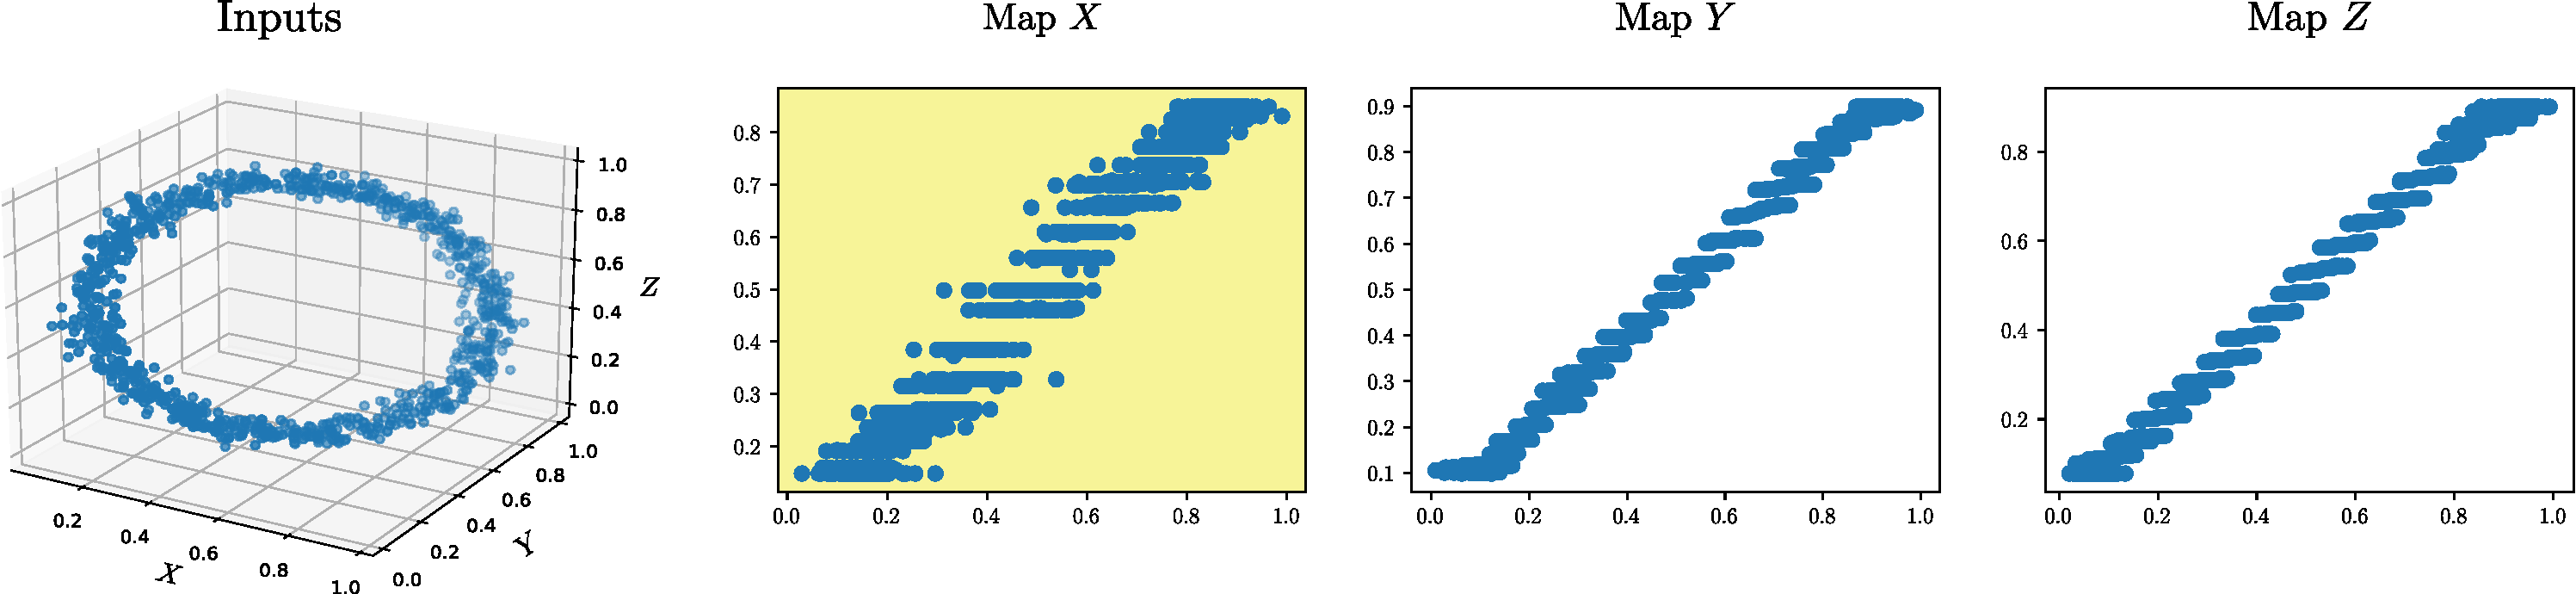
\includegraphics[width=0.9\textwidth]{pred_anneau005_inputs.pdf}
% 	\caption{\label{fig:pred_anneau}}
% \end{figure}

\begin{figure}
	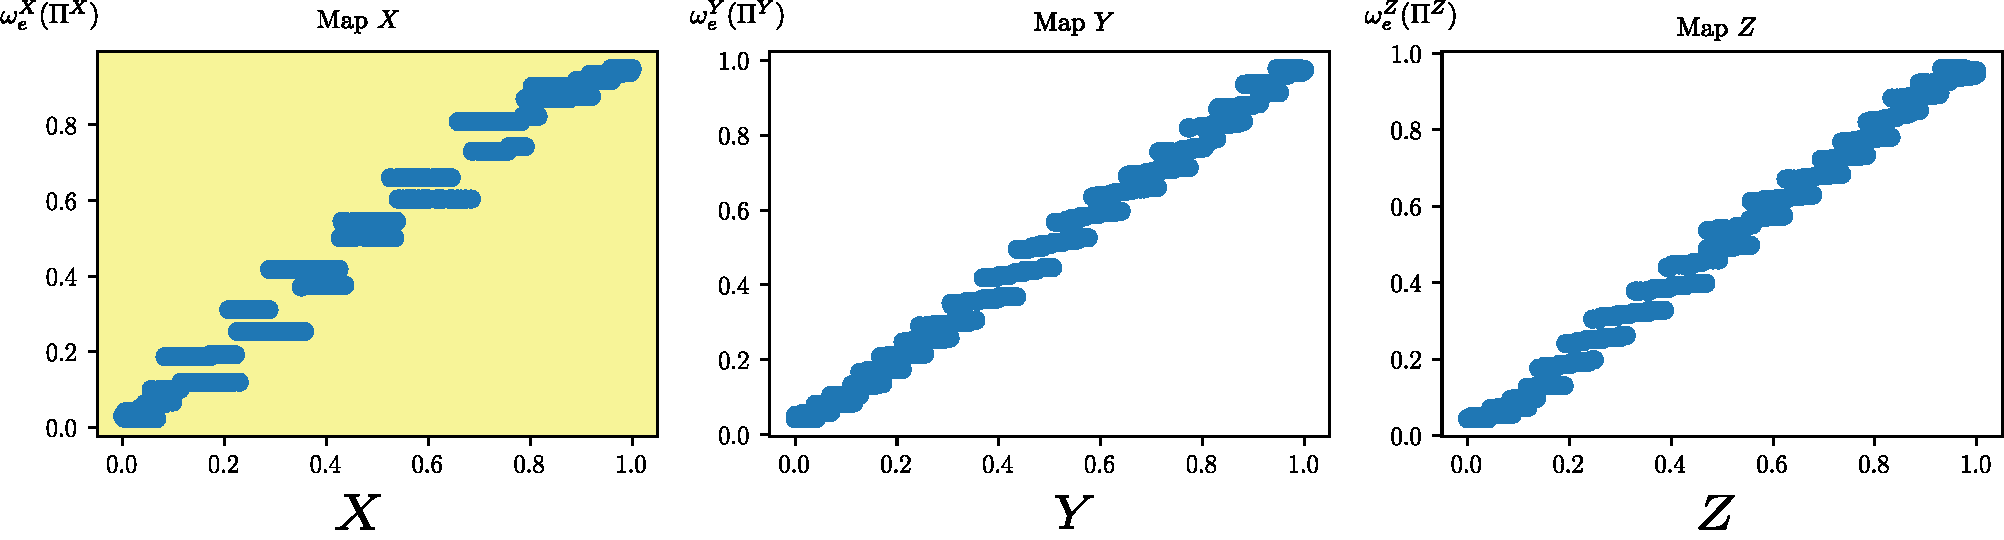
\includegraphics[width=0.9\textwidth]{prediction_x2.pdf}
	\caption{\label{fig:pred_cercle}}
\end{figure}

\begin{figure}
	\includegraphics[width=0.9\textwidth]{rceqre/prediction.pdf}
	\caption{Prédiction de l'entrée $X\m{1}$ lorsque $r_c = r_e$. Sans formation de zones, la capacité de prise de décision n'est plus possible par une carte de l'architecture. \label{fig:rcre_pred}}
\end{figure}

% \begin{figure}
% 	\centering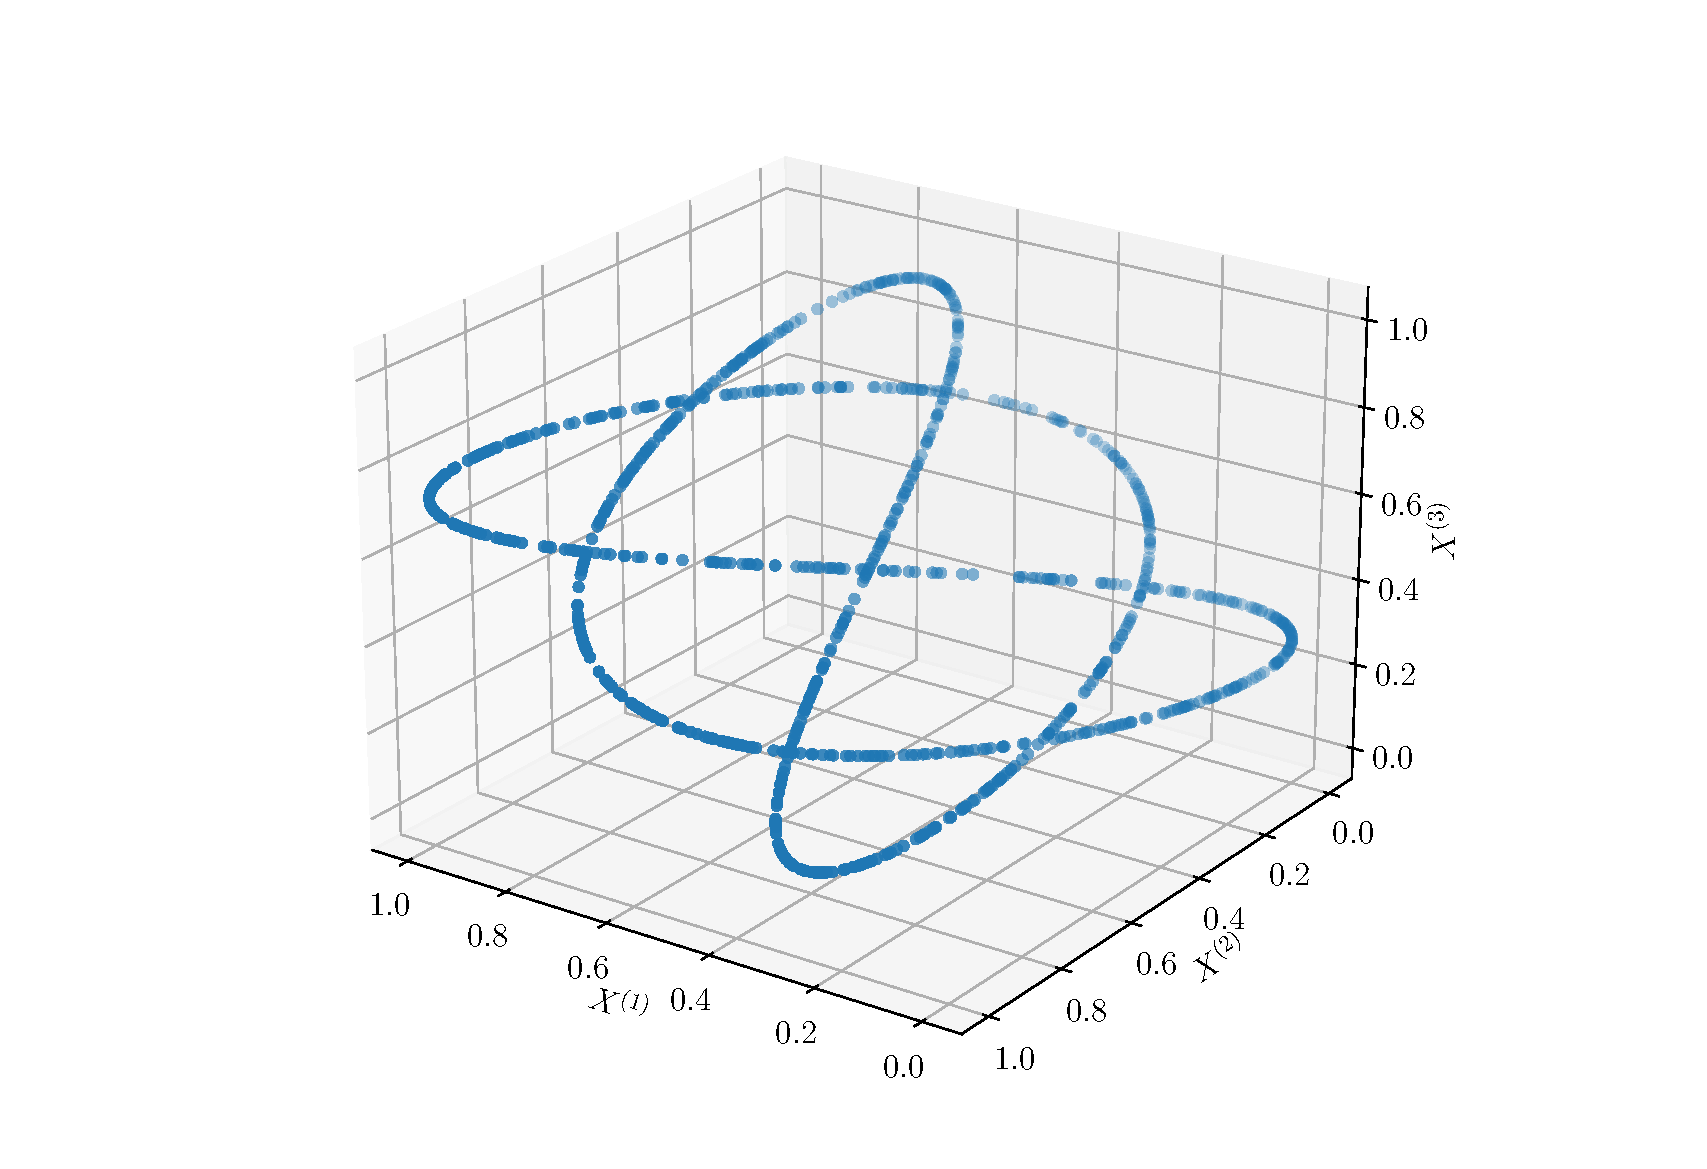
\includegraphics[width=0.5\textwidth]{lissa3D/inputs_lissa}
% 	\caption{Disposition des entrées sur une courbe de lissajous pivotée sur trois dimensions. Étant donné que la courbe est inscrite dans un plan, la connaissance de deux entrées est suffisante pour déterminer la troisième à partir du modèle.\label{fig:in_lissa_3D}}
% \end{figure}

% \begin{figure}
% \begin{minipage}{0.48\textwidth}
% \centering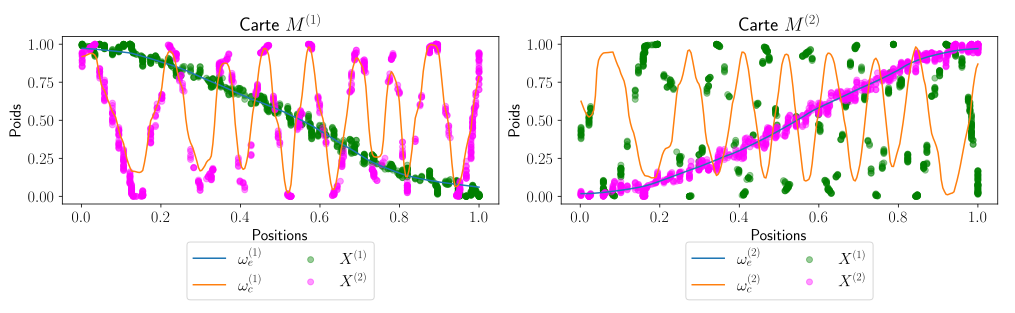
\includegraphics[width=\textwidth]{lissa3D/weights_19999}
% \end{minipage}
% \begin{minipage}{0.48\textwidth}
% \includegraphics[width=\textwidth]{lissa3D/zclosed-1-19999_error}	
% \end{minipage}	
% \caption{Représentation cartographique des poids et entrées des trois cartes après apprentissage d'une courbe de lissajous}
% \end{figure}

\begin{figure}
	\begin{minipage}{0.48\textwidth}
	\centering\includegraphics[width=\textwidth]{plan/weights}
	\end{minipage}
	\begin{minipage}{0.48\textwidth}
	\includegraphics[width=\textwidth]{plan/zclosed-1-19999_error}	
	\end{minipage}	
	\caption{Représentation cartographique des poids et entrées des trois cartes après apprentissage d'un plan pivoté en 3D et erreur de prédiction. Le découpage de l'espace par les cartes permet de prédire correctement une entrée. \label{fig:plan3}}
	\end{figure}


\subsection{Entrées réelles~: application sur un drône}

Nous sortons du cadre des entrées simulées pour nous placer dans un cas de contrôle réel.
Nous disposons d'un drône quadricoptère, commandé à distance. 
Ce drône possède une caméra frontale ainsi qu'un ensemble de capteurs internes. Chacun de ces capteurs peut être considéré comme une modalité d'un espace multimodal. \'A ces modalités s'ajoute la modalité correspondant à la commande envoyée au drône.
Le principe est d'apprendre, à l'aide d'une architecture de cartes, les relations existant entre les modalités des capteurs et de la commande afin d'ensuite prédire la commande à envoyer à partir des capteurs.
Afin que les relations entre la commande et les capteurs soient significatives, nous nous plaçons dans un cas d'application particulier~: le drône vole dans un couloir étroit, en ligne droite. Le but du drône est alors de voler en avant dans le couloir, sans toucher les murs.


Lors des expériences géométriques, les données étaient peu bruitées et nous nous étions assurés que chaque modalité contribuait à l'apprentissage du modèle. Dans cette application, les relations entre entrées sont simples, mais les données sont très bruitées et certaines entrées ne sont pas du tout déterminantes pour le modèle et peuvent ainsi polluer l'apprentissage.
Nous évaluerons ainsi la robustesse de l'algorithme à des données bruitées et la capacité de CxSOM à réagir en temps réel malgré les étapes de relaxation.

\subsubsection{Méthode expérimentale}

Le drône utilisé pour l'expérience est un quadricoptère modèle. Il possède une caméra frontale.
Nous le contrôlons à distance par un ordinateur~; la commande est réalisée en envoyant l'accélération angulaire du drône autour de ses trois axes de rotation.
Nous avons accès aux données des capteurs internes, notamment la vitesse linéaire courante selon chaque axe de déplacement. Le drône se déplace dans un couloir étroit en ligne droite, à hauteur constante et vitesse constante.

Dans le cadre de l'expérience, nous extrayons deux éléments visuels spécifiques au couloir à partir de la caméra du drône~: l'abscisse du point de fuite du couloir $x$ et la différence entre les angles des lignes du couloir, notée $\varphi$. Ces valeurs sont illustrées en figure~\ref{fig:drone}.

La commande générant le déplacement en avant (tangage) est maintenue constante. Les commandes permettant le déplacement en largeur sont alors $\omega$ et $\rho$. Dans le cadre de cette expérience, nous contrôlerons uniquement $\rho$.
Enfin, la vitesse linéaire en largeur du drône peut être récupérée à chaque instant~; nous la notons $v$.
Nous utilisons ainsi quatre modalités lors du déplacement du drône: $x$, $\varphi$, $\rho$ et $v$.
Nous construisons une architecture CxSOM sur ces quatres modalités, composée de quatre cartes connectées chacune aux trois autres.

Une phase d'apprentissage est réalisée sur des déplacements du drône contrôlés humainement. Lors de cette phase, nous avons utilisé un système de contrôle PID pour assister la commande humaine.
Cette phase d'apprentissage est réalisée hors ligne pour que les données soient présentées aléatoirement lors de l'apprentissage.
Après apprentissage, nous effectuons une phase de prédiction. Lors de cette étape, la commande $\rho$ n'est plus présentée à la carte correspondante. 
Nous envoyons alors le poids externe du BMU de cette carte comme commande du drône. Cette étape est réalisée en ligne en temps réel sur la trajectoire du drône.

La figure \ref{fig:drone_inp} présente la répartition des entrées présentées au drône. Nous avons tracé les dépendances entre chaque modalité. Nous nous intéressons ici aux dépendances entre la commande en $y$ $\rho$, sujet de la prédiction et des autres modalités.
On remarque que $\rho$ dépend linéairement de l'angle du couloir $\varphi$, mais que cette dépendance est très bruitée. 
On remarque également des dépendances entre les autres variables.

\begin{figure}
	\begin{minipage}{0.5\textwidth}
	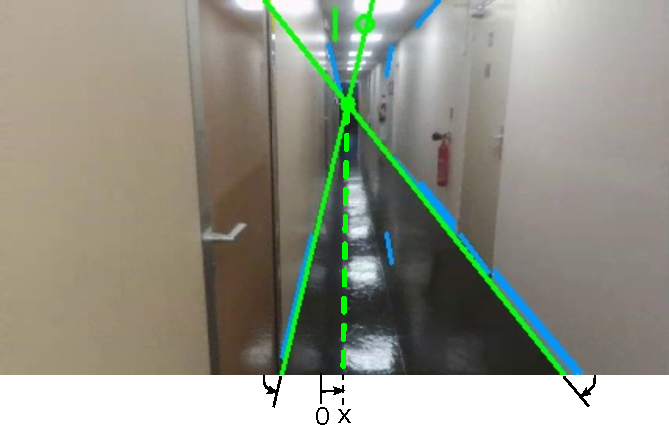
\includegraphics[width=\textwidth]{visudrone}
	\end{minipage}
	\begin{minipage}{0.5\textwidth}
	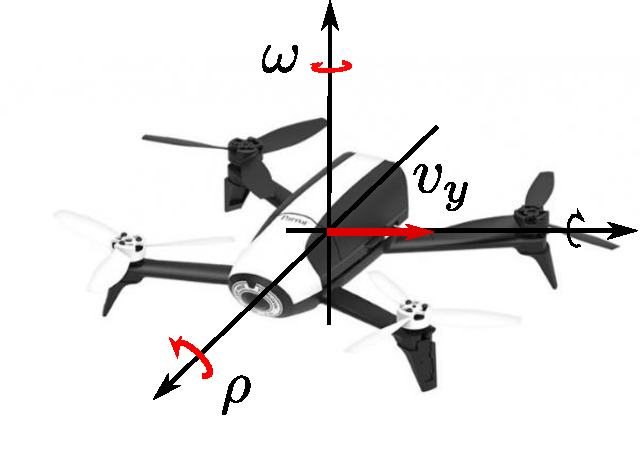
\includegraphics[width=\textwidth]{dronesteup}
	\end{minipage}
	\caption{Disposition des capteurs utilisés pour l'expérience}
	\label{fig:drone}
	\end{figure}

\begin{figure}
	\centering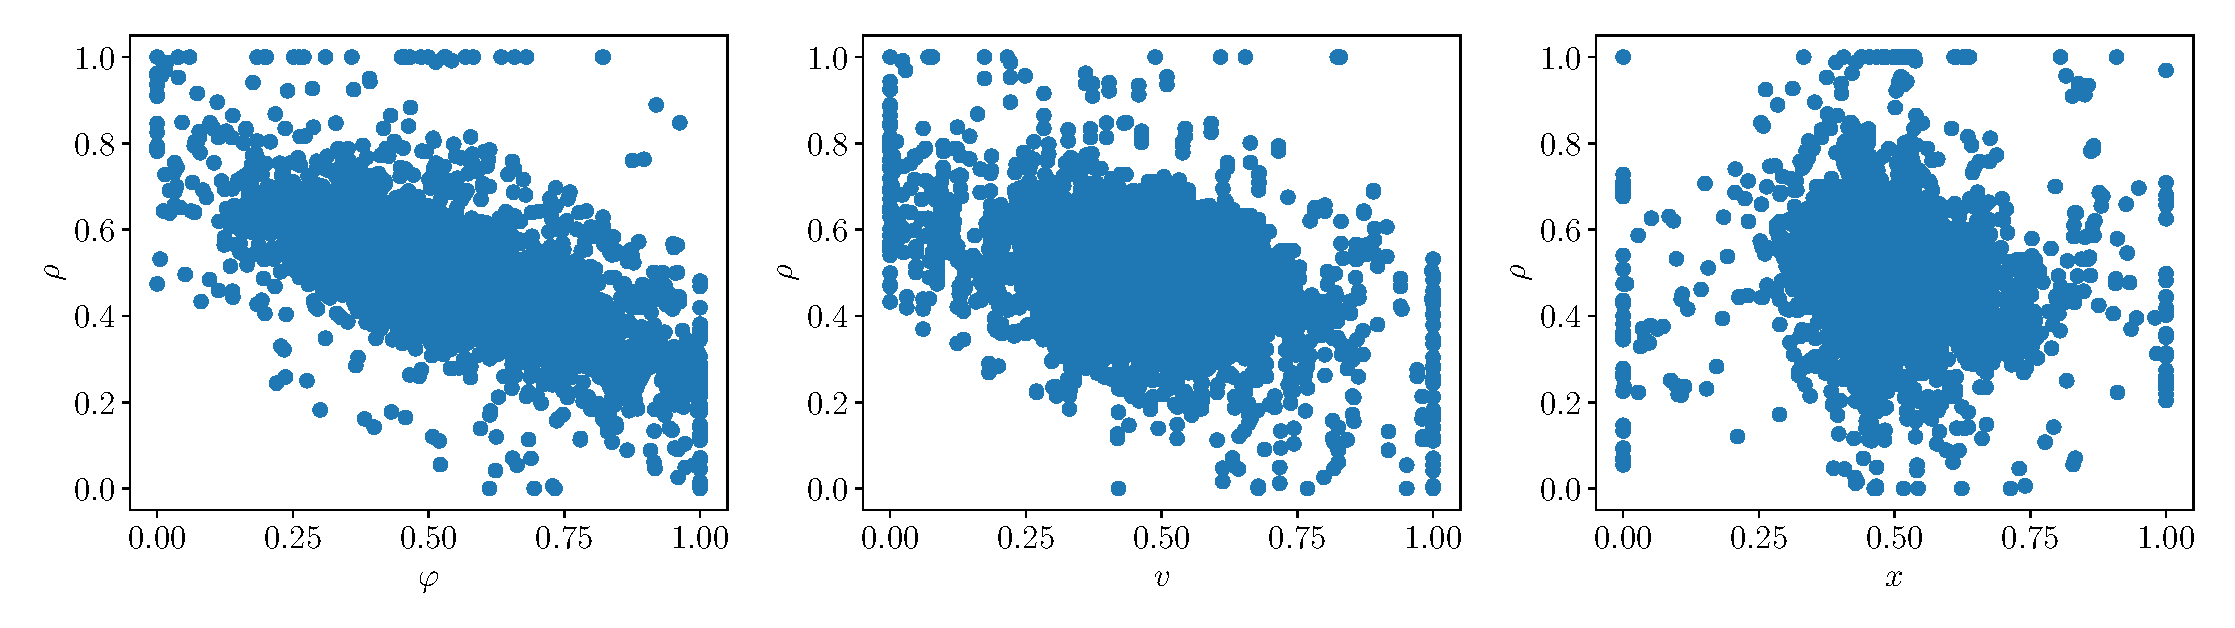
\includegraphics[width=\textwidth]{drone_inputs}
	\caption{Disposition et dépendances des entrées d'apprentissage. Nous chercherons à prédire $\rho$~: cette valeur dépend bien des autres modalités $v$, $\varphi$ et $x$. La dépendance est très simple (linéaire) mais très bruitée. \label{fig:drone_inp}}
\end{figure}

\subsubsection{Résultats}

La carte associée à $\rho$ possède donc une couche de poids externe et trois couches de poids contextuels. Ces poids sont représentés en figure \ref{fig:drone_w}. 

L'organisation des poids contextuels rappelle celle observé dans des conditions géométriques~: les poids contextuels définissent des zones. 
Contrairement à l'expérience que nous avions réalisée sur un cercle, les zones ne sont pas les mêmes selon les couches de poids contextuels.

\begin{figure}
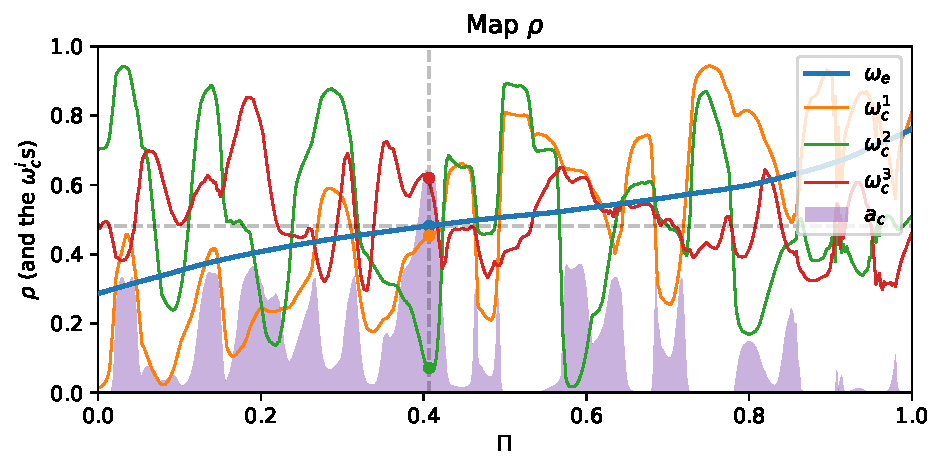
\includegraphics[width=\textwidth]{dronemap}
\caption{Disposition des poids de la carte $\rho$ après apprentissage et exemple de calcul d'activité}
\label{fig:drone_w}
\end{figure}

La phase de test réalisée en temps réel sur le drône le long du couloir montre que le drône se déplace correctement 

\subsubsection{Discussion}


Ici on ne cherchait pas à comparer avec des valeurs théorique, mais on observe que le drone ne tape pas les murs
Illustration de la capacité de prédiction et mémoire associative
Resistance au bruit
Calcul des dépendance entre les entrées et la commande:
PCA sur les entrées, calcul de MI après apprentissage

\section{Conclusion}


\ifSubfilesClassLoaded{
    \printbibliography
    %\externaldocument{../main.tex}   
}{}
\end{document}